\documentclass[12pt,A4]{report}

%########################################################################%
% TODO
%########################################################################%
% Kolla upp agency i t'nksnade maskiner
% L's chap1 Russel Norvig

% Train with certain types of food and evaluate on other types, to see how it deals with distributional shift
% Possibly add zombies that has higher probability for moving toward the agent and if contact is made a terminal state with negative reward is reached.

% bring back deep reinforcement learning

% l'sa t'nkande maskiner medvetenhet

% Why put a focus on RL


%########################################################################%
% PACKAGES
%########################################################################%

\usepackage[dvipsnames,rgb,dvips]{xcolor}
\usepackage{graphicx}
\usepackage{psfrag}
\usepackage{tikz}
\usepackage{float}
\usepackage{parskip}
\usepackage[format=plain, labelfont={bf,it}, textfont=it]{caption}

\usepackage{amsmath}
\usepackage{amssymb}
\usepackage{amsthm}

\usepackage[rflt]{floatflt}
\usepackage{latexsym}
\usepackage[Algoritm]{algorithm}
\usepackage{algpseudocode}

% for quotes 
\usepackage{dirtytalk} % \say{inline quote}
\usepackage{csquotes} % \begin{displayquote} larger quote \end{displayquote}


%########################################################################%
% REPORT STRUCTURE
%########################################################################%

\renewcommand{\chaptername}{}
\usepackage{titlesec}
\titleformat{\chapter}[hang] 
{\normalfont\huge\bfseries}{\chaptertitlename\ \thechapter:}{1em}{} 
\newcommand{\autobaj}{}
\newcommand{\autocite}{}

% Margins
\addtolength{\topmargin}{-3cm}
\addtolength{\textheight}{2cm}
\addtolength{\evensidemargin}{-1.2cm}
\addtolength{\oddsidemargin}{-1.2cm}
\addtolength{\textwidth}{2cm}
\pagestyle{myheadings}

\theoremstyle{definition}
\newtheorem*{definition*}{Definition}
\newtheorem{definition}{Definition}[section]

\usepackage{fancyhdr}

\usepackage{natbib}
% https://gking.harvard.edu/files/natnotes2.pdf

% \usepackage[american]{babel}
% \usepackage{csquotes}
% \usepackage[backend=bibtex]{biblatex}
% \usepackage[backend=bibtex, autocite=inline, sorting=none]{biblatex}
% \bibliographystyle{apa}
% \usepackage[backend=bibtex, style=author]{biblatex}
% \bibliographystyle{apa}
% \bibliographystyle{apalike}
% \usepackage[style=authoryear, autocite=inline]{biblatex}
% \usepackage{apacite}
% \bibliographystyle{apa}  \bibliographystyle{stylename}
% \bibliographystyle{apa}
% \addbibresource{ref.bib}


%########################################################################%
% TITLE
%########################################################################%

\title{Side effect minimization in Reinforcement Learning} 
\author{Jonatan Hellgren }
\date{April 2022}

\newcommand{\titel}{Impact Measurement Manager} 
\newcommand{\undertitel}{Implementing a Novel Impact Measurement Extendable to POMDP} 


\newcommand{\examina}{Jonatan Hellgren}

\newcommand{\titelsidor}{
\pagestyle{fancy}
\fancyhf{}
% \newgeometry{top=1.5cm, bottom=4cm,left=2 cm,right=1cm}
% \fancyhead[L]{
\includegraphics[width=155mm]{figures/Chalmers_GU_svart-eps-converted-to.pdf}\\}
\fancyhead[L]{
\includegraphics[width=155mm]{figures/gu_chalmers.jpg}\\}
\addtolength{\voffset}{1cm}
\renewcommand{\headrulewidth}{1pt}

%\renewcommand{\headrulewidth}{1pt}

\mbox{}
\vspace{20mm}

\noindent {\LARGE \titel}\bigskip\bigskip

\noindent {\large \undertitel}
\vspace{20mm}

\begin{center}
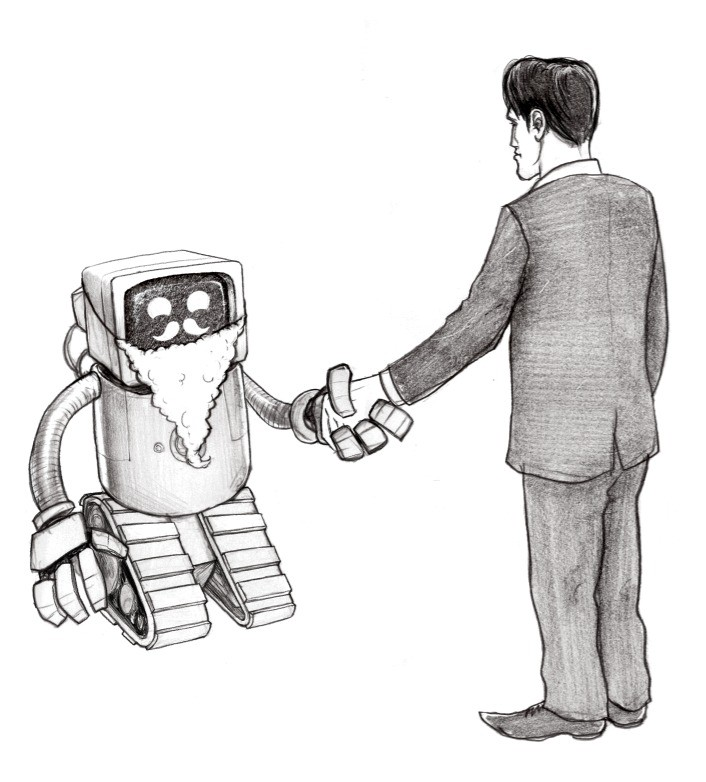
\includegraphics[scale=0.3]{figures/agreeing.jpeg}
\end{center}

\vspace{20mm}

\noindent {\large \textit{Master's thesis in Mathematical Statistics, Statistical learning and AI}} \\

\noindent {\large \examina}


\vfill
\renewcommand{\footrulewidth}{0.5pt}
\fancyfoot[L]{\vspace{0.1mm}\large %Institutionen för Matematiska vetenskaper\\
%CHALMERS TEKNISKA HÖGSKOLA\\
%GÖTEBORGS UNIVERSITET\\
Department of Mathematical Sciences\\
Chalmers University of Technology\\
University of Gothenbug\\
Gothenbug, Sweden 2022}

\newpage 
\thispagestyle{empty}
\null
\newpage
% This page is intentionally left blank.

\newpage

\thispagestyle{empty}
\begin{center}
\large Master's thesis 2022

\vspace{10mm}
{\LARGE \titel}\bigskip\bigskip

{\large \undertitel}

\vspace{10mm}
\large \examina

\vspace{5mm}
\begin{tabular}[t]{lll}
Supervisor:& Olle Häggström\\
Examinator:& Torbjörn Lundh
\end{tabular}


\vspace{30mm}
  
\includegraphics[scale=0.5]{figures/stacked_logo.png}


\vspace{5mm}
Department of Mathematical Sciences\\
Chalmers University of Technology\\
University of Gothenbug\\
Gothenbug, Sweden 2022

\end{center}

 }

\begin{document}

% \maketitle
\titelsidor


\newpage

\addtolength{\topmargin}{-1cm}
\addtolength{\textheight}{0cm}
\addtolength{\evensidemargin}{0cm}
\addtolength{\oddsidemargin}{0cm}
\addtolength{\textwidth}{0cm}

\newpage 
\thispagestyle{empty}
\null



\tableofcontents
\thispagestyle{empty}
\null

\pagenumbering{roman}

\newpage
\pagenumbering{arabic}

\pagestyle{fancy}
\fancyhf{}
\rhead{\thesection}
\lhead{\leftmark}
\renewcommand{\footrulewidth}{0pt}
\cfoot{\thepage}

% \input{1.1.txt}
%########################################################################%
% INTRODUCTION
%########################################################################%

\chapter{Introduction}
What will be covered in this report will be a small part of the big problem of creating safe Artificial Intelligence (AI). This is an issue of great importance that we should not overlook since the consequences of what we manifest in the present or near future may last for humanity's remaining history. 

What we can see today is a large focus on developing AI. With billions of dollars spent on development in 2020, while only around \$50 million on reducing the risks, see \citet{80000}. Even though the field has known about this issue since before the development of AI started. In a paper written by \citet{Turing51}, we can find the following quote:
\begin{displayquote}
  For it seems probable that once the machine thinking method had started, it would not take long to outstrip our feeble powers. There would be no question of the machines dying, and they would be able to converse with each other to sharpen their wits. At some stage therefore we should have to expect the machines to take control.
\end{displayquote}

In this introduction, we begin by defining AI. Then go through where we are today, where current progress might lead, and when we can see these changes. After that, we will cover the risks of AI that make it possibly unsafe and what is at stake. Finally, we will look at some proposed methods for creating safe AI. 

% In this introduction, we will go through some necessary background on artificial intelligence, also some arguments why concerns may be raised about its future progress. Then we will look at some paths the research is taking to avoid the potential issues that could arise with future progress. 

\section{Artificial Intelligence}
% How it works today
% * Human history is tool making, AI is a tool
% * Definitions of AI
% * Brief history 
% * Current paradigm and why it is beginning to have an impact
% * 
% * 
In recent human history, we have seen massive technological development. Human life today is in several ways different compared to how it was for millennials and even centuries ago. We can see this development as the consequence of new tools developed to extend our capability. In early prehistory, these tools were things such as fire for warmth, protection, and to cook our food which gave us more nutrition, or weapons for hunting. Later in history, these tools tend towards more complexity by automating physical labor with mechanical machines and extending the reach of the written word with the printing press. In modern times, a new tool has emerged intending to improve the thing that made all the previous tools possible, namely our intelligence. This tool is called AI and is currently starting to show its potential. 
% The idea of AI has been around since the dawning age of electronic computers. The term was first coined in \autobaj{John McCarthy et al} (1955).
% http://raysolomonoff.com/dartmouth/boxa/dart564props.pdf

The definitions of an AI vary. Although, we are now going to look at two different ones to get a clearer sense of what it is. In a standard textbook on AI education,  the authors say that the field is \say{concerned with not just understanding but also building intelligent entities - machines that can compute how to act effectively and safely in a wide range of novel situations}, see \citet[p.19]{RusselNorvig}. On \citet{Wiki}, we find another definition: 
\begin{displayquote}
Artificial Intelligence (AI) is intelligence demonstrated by machines, as opposed to the natural intelligence displayed by animals including humans.
\end{displayquote}
However, to understand this definition properly it is necessary to define what intelligence is. In \citet[p.22]{TankandeMaskiner} the author brings up the following to clarify this: \say{the quality that enables an entity to function effectively and with foresight in its environment} and \say{the ability to correctly perceive one's surrounding environment and act in a way that maximizes one's chances of achieving given goals}. So, the AI definition remains rather broad.
% https://en.wikipedia.org/wiki/Artificial_intelligence

\subsubsection{AI Paradigms}
We create ordinary computer programs by giving a computer step-by-step instructions. If we execute this program, it performs the desired task, such as calculating digits of $\pi$ or launching a web browser. This method was also the case for the first two paradigms of AI: rule-based AI and expert systems where humans explicitly programmed their knowledge into the computer to create automation, see \citet[c.1]{Bostrom14}. The systems made in such a way are typically suited for less complex tasks where it is possible to model the entire behavior explicitly by handpicking the parameters. These systems are typically called good old fashion AI. 

However, in the current machine learning paradigm, the approach is to specify an objective function that captures what we want and then use an optimizer to train the AI until it solves the task. This approach focuses more on what should be solved instead of how it should be solved, which allows for automation in a more complex task where explicitly defining the behavior in every situation is infeasible because it is too big or complex. 

In recent years, AI has been applied in the industry more broadly, and it is already generating yearly revenue of trillions of dollars, see \citet[p.19]{RusselNorvig}. This progress has become possible due to more available data, faster computer hardware, and increased funding for research. 

\subsubsection{Intelligent Agents}
Although these systems are highly automated, a key point here is that these systems still require humans to create and function. However, the development of AI is shifting the tool to a more automated one. With this trend, AI systems are developing into intelligent agents. An agent acts or, more specifically, can:
\begin{itemize}
  \item operate autonomously,
  \item perceive the environment,
  \item persist over a prolonged period,
  \item adapt to change,
  \item and create and pursue goals.
\end{itemize}
The reason why this is attractive is that the human intervention part required by an AI system is likely to become a bottleneck.
% , see \citet[\textbf{PAGE}]{TankandeMaskiner}.

Reinforcement Learning (RL) is a field of machine learning that creates intelligent agents. However, it is not the only method for creating intelligent agents. RL differentiates from other machine learning techniques by being a more exploratory approach where the agent learns by trial and error. The method is similar to how one goes about training a pet, where desirable behavior receives a positive reward and undesired behavior gets a negative. In such a way, the agent develops a behavior. 

In recent years, RL has seen substantial development with advances in board games such as go in \citet{Silver}, autonomous vehicles in \citet{Levinson}, and video games in \citet{Minh}. These advancements display the usefulness of these agents and motivate the possibility of implementation in our daily life. RL will be the main focus of this report. 
% Levinson et al. https://ieeexplore.ieee.org/abstract/document/5940562?casa_token=pxjrsi7VJZ8AAAAA:MNQmlmsfHVJ8VdW9jNlZzHPnS4gBTk4q6yCx_AFsF-rRheHnP9C2CrjvaWt0vD9C0oWfgt8o
% Minh et al: https://arxiv.org/pdf/1312.5602.pdf
% Silver et al. https://www.nature.com/articles/nature16961%7D



\subsection{Future Progress}
% Explain what we are aiming at in the future
When the pioneers of AI started the development, the ideas were not only to apply systems that automate a narrow set of tasks, as we can see in modern AI systems. The idea was instead to recreate the intellect of a human in a machine, see \citet{Dartmouth}. Doing this, would extend our thoughts from mere thoughts to a new kind of intelligence running on silicon-based hardware instead of carbon-based wetware. This concept is called Artificial General Intelligence (AGI) - an AI that can solve an arbitrary set of tasks with as good or better performance as a human. The main difference from AI is that the set of tasks is no longer narrow and bounded. %An even more advanced AGI is often called \textit{superintelligence} - an AI that is much smarter than a human in all possible domains. \autobaj{Superintelligence} 

% RL for acheiving AGI, why not and why it is still worth to study it as if it was going to become AGI

% Example of an AGI
An example of a current AI system is DeepMinds AlphaMu, which can play board games, and video games. Recently, the researchers at DeepMind used the same technique to create a video compression better than the current methods used for the task, see \citet{Mandhane}. The techniques used in this system originate from the famous AlphaGo, see \citet{Silver}, which won against the Go grandmaster Lee Sedol in the game of Go, see \citet{DeepMind}. Although AlphaMu presents an impressive performance in multiple tasks, it still can not be considered an AGI since each new task require engineering effort. On the other hand, an AGI would, in theory, be able to pick up any task and perform it at a human level or better without any new human intervention.
% https://arxiv.org/pdf/2202.06626.pdf
% https://www.deepmind.com/research/highlighted-research/alphago/the-challenge-match
% https://www.deepmind.com/blog/muzero-mastering-go-chess-shogi-and-atari-without-rules

% consequences of AGI
The significant difference with this shift is that it will increase the possible tasks that a single system can perform. The possible set of tasks would become arbitrary. The implications of such a breakthrough would likely be on the same scale as the industrial revolution, if not greater, see \citet{CritchKruger}. However, instead of automating physical labor as the industrial revolution did, it will automate mental labor. 


% Computers can recall more information and process information faster then humans
\subsubsection{Is an AGI Possible?}
A reason to believe that such systems are possible to build is that we know that human intelligence evolved naturally with evolution, so something similar should be possible to reproduce in machines. An argument against this is substance dependence, see \citet{Bostrom03} - to believe that intelligence or consciousness can only occur in carbon-based life forms and not in silicon-based, caused by inherent or other properties. 

 %Created intelligence could become more intelligent than us since intelligence might not have been selected for by evolution \autobaj{S. Legg} and when we develop AI, we can focus the development specifically on intelligence. 

Regarding intelligence, there is no longer any reasonable argument for it. However, the question of consciousness, although an interesting question, can be seen as irrelevant when considering what actions an AI makes since the consequence is still the same. Or as it is explained in \citet[p.22]{HumanCompatible}: 
\begin{displayquote}
  Suppose I give you a program and ask, 'Does this present a threat to humanity?'. You analyze the code and indeed, when run, the code will form and carry out a plan whose result is the destruction of the human race, just as a chess program will form and carry out a plan whose result will be the defeat of any human who faces it. Now suppose I tell you that the code, when run, also creates a form of machine consciousness. Will that change your predictions? Not at all. It makes \textit{absolutely no difference}.
\end{displayquote}
% S. Legg Machine Super Intelligence
% Bostom Are we living in a computer simulation

Developing a AGI is not an easy task. However, it might not be necessary to create one directly, see \citet{Bostrom14}. A different approach is to create an AI system that can develop a AGI system. A fundamental property of this AI system is self-improvement. Theoretically, if an AI system has reached a threshold where it becomes better at improving itself than its creators, then letting the AI create the next version of itself, this self-improvement quality would improve. If this iterative process keeps going, it can create an intelligence explosion called the singularity, as discussed in \citet{Yudkowsky13}. 

Although the author states that it is not certain that this will happen fast enough to be considered an explosion since intelligence might not be so easy to create once we have collected all the low-hanging fruits, which could yield a deceleration in the development. Also, perhaps intelligence is more difficult to create then we think, and we need whole new method for going beyond human intelligence.
% https://intelligence.org/files/IEM.pdf
% ”If this iterative process keeps going, it will create an intelligence explosion…”. Detta är förhastat. Såvitt vi vet finns inga garantier för att processen går så fort att den förtjänar benämnas explosion. Ett annat möjligt scenario är att effekter av typen ”alla lågt hängande frukter har redan plockats” skapar en inbromsning. Yudkowsky (2013) behandlar denna problematik ingående, eller se Kapitel 4 i Tänkande maskiner för en mer summarisk behandling. 
% Why consciousness may matter
% capability for generating suffering
% if impossible, then mind uploading will seem a lot less interesting

\subsubsection{Impacts of AGI}
The following quote by I.J. \citet[p.33]{IJGood} summarizes the potential impacts of an AGI: 
\begin{displayquote}
Thus the first ultraintelligent machine is the last invention that man need ever make, provided that the machine is docile enough to tell us how to keep it under control
\end{displayquote}
This quote presents a dichotomy since we will either not be able to compete with creating novel inventions or not be able to preserve our existence. Reasons for the latter we will come back to in later sections. 

% superintelligence quote
% https://en.wikipedia.org/wiki/I._J._Good
% AGI is not required to see this shift, here are other definitions
An AGI breakthrough is probably unnecessary for AI to impact on the same scale as the industrial revolution. Because all things we deem as intelligent would not help for this purpose. For example, physical motor skills, food digestion, and blood pressure regulation are examples of intelligent things our brain does that are hard to connect to how an AI could use to impact the world. However, a more narrow set of intelligent behavior could exist that could have an impact. 

For example, let us assume there exists an AI with a superhuman ability to create convincing and motivating speeches. Then someone could abuse this technology to become the president or prime minister in a high-influence country. Then the possible bad outcomes that could happen would be many, mainly because it can be someone incompetent, but also if the person keeps consulting the AI for advice since we would rely on the AIs drives, which are unknown. 
%Finance is another field where AI could impact. By steering the world's funding towards its specific goals or crashing the price for something it wants to purchase. 

For this reason, many researchers have stopped talking about AGI and have refined the concepts, see \citet{CritchKruger}. An AI system capable enough to induce transformative consequences on the same scale as the industrial or agricultural revolution is called an \textit{transformative AI} (TAI). On the other hand, if a \textit{transformative AI} once deployed would be unstoppable, it is instead called an \textit{prepotent AI}. 
% CRITCH KRUGER, KATJA CRACE SURVEY


\subsection{Timeline for Transformative AI Breakthrough}
% Timeline for when we can see this, first how to estimate it
The well-known AIs of today still have not reached the levels required for a TAI. For example, AlphaStar, an AI that won against world champions in the complex computer game DotA 2, see \citet{ALphaStar} is estimated in terms of total computational power to be \say{about as sophisticated} as a bee. While the language generator model GPT-3 that can summarize, continue, and carry out convincing conversations is estimated to be \say{more sophisticated} than a bee, see \citet{Ajeya}.
% https://www.deepmind.com/blog/alphastar-mastering-the-real-time-strategy-game-starcraft-ii

Although, it is important to point out that this is not a direct comparison. For example, GPT-3s social and pollen finding skills is not impressive compared to a bee. Similarly, if we tasked a bee to summarize text, its abilities would not be impressive. Intelligence is not one-dimensional. Instead this comparison means is that the computational power is about the same. 
% intelligence can not be measured with only computational power, since the intelligence of theses AI-system is vastly different compared to biological lifeforms. 

The question of when we will see these breakthroughs in the field that enables TAI systems is hard to answer, but with the worldwide increase in funding and research, we are undoubtedly getting closer. There have been attempts to answer this question, and the results of a survey and a more quantitative forecasting model will now be covered. 
% https://www.nature.com/articles/d41586-020-03409-8

% survey result
\subsubsection{Survey Results}
In a well-cited survey \citet{Grace}, they asked researchers in the field of AI to estimate the probability of human-level machine intelligence (unaided machines that can achieve all tasks better and more cheaply than human workers) arriving in the future years. The conclusion of the survey where:
\begin{displayquote}
Researchers believe there is a 50\% chance of AI outperforming humans in all tasks in 45 years and of automating all human jobs in 120 years, with Asian respondents expecting these dates much sooner than North Americans.
\end{displayquote}
Although, this result should be taken with a grain of salt since the distribution of answers had high variation. As well as, there should not be such a big difference between solving all tasks and all jobs since a job consists of a set of tasks, and thus if one can perform every task performing every job should be possible. There is still something we can take away from this survey about the timeline, namely that researchers mostly think AI can automate all tasks within this century. Also, it tells us how unsure the research field is about when this will happen. 

\subsubsection{Forecasting Model}
Another approach for predicting when TAI systems will be possible to train is a quantitative forecasting model, see \citet{Ajeya}. This model uses biological anchors to estimate how much computing is necessary for the training. In the model, they base the biological anchors on factors that played a role in the development of human intelligence. For example:
\begin{itemize}
  \item the amount of information in our genome, 
  \item the computational power in our brain,
  \item and all the computational power available on our planet. 
\end{itemize}
Each anchor is then assigned a weight according to how likely the author believes them to be. Then using parameters such as rate of development in hardware, algorithmic progress, and willingness to spend money, they estimate how likely a TAI development is for any given year in the future. 

The results are a wide Bayesian probability distribution estimating the probability of the possibility of training a TAI. This distribution is summarized in \citet{an121} the following way:
\begin{displayquote}
For the median of 2052, the author guesses that these considerations roughly cancel out, and so rounds the median for the development of TAI to 2050. A sensitivity analysis concludes that 2040 is the “most aggressive plausible median”, while the “most conservative plausible median” is 2080.
\end{displayquote}
Comparing the results of the forecasting model with the survey is not straightforward since they answer slightly different questions. However, both conclude that we will likely see the development of TAI being possible in this century.

There is one thing worth mentioning when considering timelines for future TAI. It is not necessarily true that the amount of progress will continue to develop at the current rate. The field of AI has previously been through two winters where the funding and excitement decreased, see \citet[p.42]{RusselNorvig}. The reason is mainly due to unmet high expectations. So if a third winter happens, which is possible, we could expect the rate of development to decrease. On the contrary, the progress could significantly increase due to breakthroughs in relevant fields and thus shorten the timeline.

% Giving us what timeline to solve the problem?

\subsection{Basic Drives}
% One might argue that if an AI described in the previous section were intelligent it wouldn't have acted in the way described, because it would have been stupid and not intelligent at all. But that argument assumes that the system would have common sense, as most of us do, but for an AI it is not sure that common sense will be common. That leads us to the question, what does an AI want?
Knowing what impacts a potential TAI or AGI will cause is hard without understanding how it will behave. There is research about the foundations for understanding the possible behavior by hypothesizing what drives it could have. A commonly adopted view (but still controversial, see \citet{MullerCannon} for criticism and \citet{Haggstrom21} for a response) is the Omohundro-Bostrom theory for AI driving forces, described in \citet{Haggstrom19}. Two cornerstones imply it, namely \textit{instrumental convergence thesis} and the \textit{orthogonality thesis}, which we will now explain further.
% https://onlinelibrary.wiley.com/doi/full/10.1111/rati.12320
% Challenges to the Omohundro—Bostrom framework for AI motivations
% http://www.math.chalmers.se/~olleh/ChallengesOBframeworkDeanonymized.pdf

% Olles response
% http://www.math.chalmers.se/~owww.math.chalmers.se/~olleh/ChallengesOBframeworkDeanonymized.pdf lleh/ChallengesOBframeworkDeanonymized.pdf

\subsubsection{Instrumental Convergence}
In the current paradigm, the creator of the AI agent assigns it a goal. We call this goal the terminal goal since it completes the task. This task could be anything, for example, maximizing the number of paper clips produced by a factory, finding decimals in $\pi$, or counting all the blades of grass on our planet. According to instrumental convergence during the agent's pursuit of the terminal goal, naturally, other instrumental goals emerge. Examples of such would be:
\begin{itemize}
    \item Self-preservation: keeping it self up and running will let the agent make sure its goals are met.
    \item Self-improvement: by updating and improving it self, the agent will be better able to complete its goal.
    \item Discretization: if the agent would suspect that the pursuit of its goal would be hindered by another entity such as a human. Then it could be a good tactic to make sure no one knows it is pursuing its goals, until it is certain that it can be acheived.
    \item Goal perseverance: keeping its final goal intact,
    \item Resource accumulation: since more resources will likely yield more power,
\end{itemize}
see \citet{Omohundro08}. This theory was later named the \textit{instrumental convergence thesis} in \citet{Bostrom12}. Originally without the third point \textit{discretization}, which later got added in \citet{Bostrom14}.

These instrumental goals help the agent pursue its terminal goal and will likely help other agents with a wide range of different terminal goals. Thus many different agents would converge to this set of instrumental goals, hence the name. However, there are some examples where the terminal goal does not benefit from these instrumental goals. For example, if the terminal goal is to kill itself or do nothing, this set of instrumental goals would not emerge. 

% https://selfawaresystems.files.wordpress.com/2008/01/ai_drives_final.pdf

Still, it does not yet exist any rigorous mathematical proof for this. However, some work has been trying to lay the necessary foundations for it, see \citet{Turner19a}. In the paper, the authors prove in basic environments that some actions give the agent more power in the sense that more possible future actions become available. On average, on multiple tasks in the same environment, they found that those actions that yield higher power were also optimal. Hence, we can see instrumental goals as a tendency to seek power.
% https://arxiv.org/pdf/1912.01683.pdf

% LÄS
% https://www.emerald.com/insight/content/doi/10.1108/FS-04-2018-0039/full/pdf?title=challenges-to-the-omohundrobostrom-framework-for-ai-motivations

\subsubsection{Orthogonality Thesis}
The orthogonality thesis is described as \say{More or less any final goal is compatible with more or less arbitrarily any level of intelligence}, in \citet{Bostrom12}. To avoid counterexamples that combine low intelligence with an advanced goal, we can change \say{any level of intelligence} to \say{arbitrary high level of intelligence}, see \citet{Haggstrom19}. With this, there exist some counterexamples. For example, if we gave an intelligent AI the goal of being stupid, then the AI would not be so intelligent.

A contrary belief is that all intelligent AIs will converge on the same goal due to their intelligence. Although, for humans, this belief is natural since most humans have similar goals. Nevertheless, when considering the potential risks, this scenario would be alarming since it would be impossible to control all sufficiently intelligent AIs. The consequences of the Bostrom-Omohundro theory will be brought up in the following section once we have covered a bit more about AI safety.

% An intelligent AI could have a stupid task from our point of view, such as counting all the blades of grass on our planet, or it can have a goal that we may deem as an important one, like keeping the climate on earth habitable for the species that currently live on it. For an AI each task would be as important, given that we assigned the goal to it during its creation.
% https://www.nickbostrom.com/superintelligentwill.pdf

% If it is true it present possibly terrible consequences, only considering current goal
% still controverisal and there exists some counter arguments


\section{AI Safety}
% What we are doing today is not going to solve this issue
It is possible to use tools in multiple ways. Some uses might be well-intentioned, while others are ill-intentioned. For example, one can use a hammer to build a house and hit another person. The same is the case for AI because it still is a tool. Although, the consequences might be more severe and possibly even pose an existential risk to humanity since the power is much greater. Where an existential risk is described in \citet{FLI} as:
\begin{displayquote}
An existential risk is any risk that has the potential to eliminate all of humanity or, at the very least, kill large swaths of the global population, leaving the survivors without sufficient means to rebuild society to current standards of living.
\end{displayquote}
% https://futureoflife.org/background/existential-risk/

When thinking about this, the main concerns might mainly be on ill-intentioned use, and indeed creating automated killer robots can lead to existential consequences. However, a well-intentioned use might also pose a potentially existential risk, for example, when the AI system develops a destructive method for achieving its goal. 

The causes for the possibility of existential risk occur in well-intentioned use we will cover in this section. Firstly by defining safe AI. Secondly, we will look at the consequences proposed in the literature that can arise if we make an unsafe AI system. Finally, we will cover three current approaches for creating safe AI. 
% and what problems could arise if we fail to make it.
% https://futureoflife.org/background/benefits-risks-of-artificial-intelligence/

% "Let's just have humans monitor the AIs and have humans make the final decision."
% "Well, we can't really do that because we don't have enough humans. And even if we stopped AIs from making decisions until humans can check, all economic incentives point in the other direction."
% "...for all its protestations that it would always keep a human in the decision-making loop, the Pentagon is, unsurprisingly, inevitably, sliding towards fully autonomous drone warfare as the next technological step to maintain military superiority over Russia & China."

\subsection{AI Alignment}
% \begin{itemize}
  % \item AI alignment as an aproach for safe AI
  % \item Clarifying alignment, inner and outer
  % \item Explain figure
% \end{itemize}

% RL, tricky to create reward function, since it is hard to predict what behavior it creates

A big part of creating a safe AI is AI alignment, which refers to the goals of the AI being in line and not conflicting with the intended goal. Therefore, an AI that does something at cross-purposes to the intended goal is called unaligned. In \citet{Hubringer}, the authors split AI alignment into two parts: \textit{intent alignment} - the alignment of the human intent with the AI's action, and \textit{capability robustness} - an AI system's ability to perform well in environments different from the training environments. 
% Clarifying alignment
% https://www.alignmentforum.org/posts/SzecSPYxqRa5GCaSF/clarifying-inner-alignment-terminology

In the current machine learning paradigm, intent alignment further breaks down into two parts: \textit{inner} and \textit{outer alignment}, when going from human intent to the agent's actions. Because in machine learning, we use an algorithm to optimize the parameters for a model that later optimizes the objective function. In Figure \ref{fig:alignment}, we can see a visual representation of this intent alignment. In the context of RL, the agent is an optimizer that maximizes its reward, but as we can see in the figure is itself optimized by another optimizing algorithm. This makes the agent a \textit{mesa optimizer}, where the word \textit{mesa}, is greek for inside. 

\begin{figure}[H]
  \centering
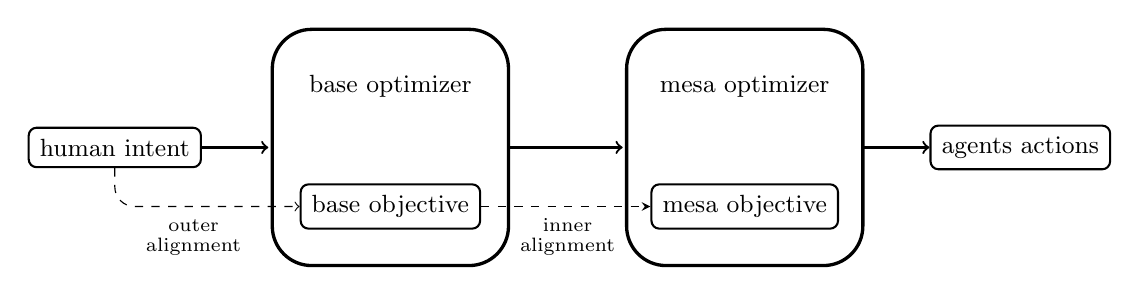
\begin{tikzpicture}[
  % GLOBAL CFG
  font=\scriptsize,
  % Styles
  cell/.style={% For the main box
      rectangle, 
      rounded corners=5mm, 
      draw,
      very thick,
      },
  operator/.style={%For operators like +  and  x
      circle,
      draw,
      inner sep=-0.5pt,
      minimum height =.4cm,
      },
  function/.style={%For functions
      ellipse,
      draw,
      inner sep=1pt
      },
  ct/.style={% For external inputs and outputs
      rectangle, 
      rounded corners=1mm, 
      draw,
      line width = .75pt,
      minimum width=1cm,
      inner sep=4pt,
      },
  gt/.style={% For internal inputs
      rectangle,
      draw,
      minimum width=10mm,
      minimum height=6mm,
      inner sep=1pt
      },
  empty/.style={% Empty nodes for joining arrows
      rectangle,
      draw,
      minimum width=0mm,
      minimum height=0mm,
      inner sep=0pt
      },
  mylabel/.style={% something new that I have learned
      font=\scriptsize\sffamily
      },
  ArrowC1/.style={% Arrows with rounded corners
      rounded corners=.25cm,
      thick,
      },
  ArrowC2/.style={% Arrows with big rounded corners
      rounded corners=.5cm,
      thick,
      },
  ]
    
    %Start drawing the thing...    

  % Draw the cell: 
  \node [cell, minimum height =3cm, minimum width=3cm] at (0,0){} ;
  \node [cell, minimum height =3cm, minimum width=3cm] at (4.5,0){} ;

  \node [empty, label={\small base optimizer}] (name1) at (0, 0.5) {};
  \node [empty, label={\small mesa optimizer}] (name2) at (4.5, 0.5) {};
  \node [empty, label={outer}] (name2) at (-2.5, -1.2) {};
  \node [empty, label={alignment}] (name2) at (-2.5, -1.5) {};
  \node [empty, label={inner}] (name2) at (2.25, -1.2) {};
  \node [empty, label={alignment}] (name2) at (2.25, -1.5) {};

  \node [ct] (human) at (-3.5, 0) {\small human intent};
  \node [ct] (acts) at (8, 0) {\small agents actions};

  \node [ct, minimum width=2cm] (optim1) at (0,-0.75) {\small base objective}; 
  \node [ct, minimum width=2cm] (optim2) at (4.5,-0.75) {\small mesa objective}; 
  
  \draw [dashed,->,style={rounded corners=.25cm}] (human) |- (optim1);
  \draw [dashed,->] (optim1) [-stealth] -- (optim2);

  \draw [->, thick] (human) -- (-1.55,0);
  \draw [->, thick] (1.5, 0) -- (2.95,0);
  \draw [->, thick] (6, 0) -- (acts);

\end{tikzpicture}

  \caption{Here we can see a visual representation of how human intent connects to the agent's actions. The two optimizers each optimize their objective. The dashed arrows show the connection the different kinds of alignment has on the objectives of the optimizers.}
  \label{fig:alignment}
\end{figure}

The main focus of this report will be on outer alignment, so that is where we will focus. Nevertheless, since methods for dealing with one might affect the others, we can not consider them isolated problems. Thus we will also cover inner alignment.


% Solving intent alignment further breaks down into two obstacles in the current paradigm of machine learning. When going from human intent to the agents actions, both of these obstacles are causes for information to be lost about the true objective. The obstacles are called , they are defined in the following way:

\begin{displayquote} 
\textbf{Outer alignment.} 
  Outer alignment is the alignment between the base objective and the \textit{human intent}. We can achieve this with a reward function that correctly captures what the agent \textit{should} do and what it \textit{should not} do.
\end{displayquote} 

\begin{displayquote} 
  \textbf{Inner alignment.} 
Inner alignment is the alignment between the \textit{mesa objective} and the \textit{base objective}. In the context of RL, we can achieve this when the agent captures the intent in the reward function.
\end{displayquote} 

% 11 proposals
% https://arxiv.org/pdf/2012.07532.pdf

% Risks from learned optimization
% https://arxiv.org/pdf/1906.01820.pdf


% This might seem as a easy problem, we just need to be precise what we want it to do and things should be fine. However, foreseeing all the possible ways an might go about to pursue a goal will become very hard once they become smarter then us. 

% One reason for expecting it to be a hard problem is that we still are not sure about the basic drives it might have, as discussed in the previous section. Predicting the direction it will take once deployed thus becomes strikingly difficult.
% In \autobaj{Amodei et al.} the field of AI safety in to five different parts and suggested research directions for each of them. A similar outline will be provided in this report. 


% \subsubsection{Reward hacking} 
% \subsubsection{Scalable oversight}
% \subsubsection{Safe exploration}
% \subsubsection{Robustness to distributional shift}
% \subsubsection{Negative side effects}


% Risks from Learned Optimization in Advanced Machine Learning Systems

% In recent years we have seen some examples of how AI can have negative side effects. For example the algorithmic bias we can see in models used by lawyers to determine how long of a sentence a felon would receive after committing a crime, it was shown that the models gave people with darker skin a significantly longer imprisonment\autobaj{Karen Hao}. Another one is that social media exploits our psychology with the help of AI to get our attention and keep us engaged. 
% https://www.technologyreview.com/2019/01/21/137783/algorithms-criminal-justice-ai/

% These problems are alarming since if we have a problem with the AI of today, how severe might future problems be with more powerful AIs that also might be applied more broadly. Several AI researchers have raised warnings for future development of AI, Stuart Russel, Max Tegmark, Eliezer Yudkowsky to name but a few. \autobaj{K"LLOR}

% example of existential risk, conflicting goals
% factory accidentally improves their AI to super-intelligent levels. 
%As for how such scenarios could play out a common example is the \textit{paperclip armageddon}. In which a paperclip maximizer is made super-intelligent and starts accumulating resources such as hardware and money. Eventually, the paperclip maximizer comes to a point where the existence of humans serves no purpose or possibly even has a negative effect on producing paperclips, and thus they become extinct.

% concrete problems in AI safety Amodei et al
% some more immediate issues: unemployment, misuse of machine learning,
% long term issues, how will we see the machines we create if they become conscious. Existential risks of AI.
\subsection{Unaligned AI}
Creating safe AI is hard, mainly since humans evolved to understand other humans, not computers. In a speech by Eliezer Yudkowsky, he explains that this becomes a problem because it will be able to find solutions we can not think about since it can look for solutions in a completely different and possibly larger solution space, see \citet{Yudkowsky16}. For this reason, AI can have unintended consequences we can not even consider a possibility. 

In addition to the difficulty of specifying a proper reward function, side effects may also arise as unintended consequences of proper optimal behavior. In \citet{Saisubramanian} they state that side effects:
\begin{displayquote}
  ... occur because the agent's model and objective function focus on some aspects of the environment but its operation could impact additional aspects of the environment.
\end{displayquote}
% To avoid negative side effects one has to in the objective function specifically state what the agent should not do.
% https://ojs.aaai.org/index.php/aimagazine/article/download/7390/18881

When an AI impacts the environment in a way that is unnecessary for achieving its objective, we consider it a side effect, see \citet{Amodei}. An example is if an AI agent's task is to navigate a room and the fastest path knocks over a fragile object that would break on impact with the floor. Then breaking the fragile object would be considered a side effect since it is not required to complete its task, as long as the agent has enough space to walk around it. 
% https://axrp.net/episode/2021/05/14/episode-7-side-effects-victoria-krakovna.html

The problem of side effect avoidance is related to the frame problem described in \citet{Mc69}, which describes the difficulty of logically describing the consequences of an action without having to define many axioms about how the environment functions. For example, if a robotic arm is stacking boxes, we need to define things such as the boxes can not intersect and instead collide upon impact. Also, a box only moves when picked up, and so on. The list grows large quickly. Eventually, we would need to describe things on a molecular scale.

Similarly, each action can have many side effects, and it is impractical to state everything that can happen and explicitly penalize all the unwanted ones. Consequently, we often know what we want the agent to do, but it can be hard to specify what we do not want it to do, in addition, to the difficulty of knowing what side effects might occur.
% Om du skall nämna “the frame problem” bör du kort tala om vad det är, samt också vari sambandet med side effects består. Som det nu ser ut väntar sig läsaren att meningen ”Each action can have…” är (början på) en förklaring av dessa saker, men så verkar inte vara fallet (väl?).


\subsubsection{Reward Hacking}
% \subsubsection{Outer alignment}
As mentioned earlier, one creates the behavior of an AI agent by defining a reward function. A reward function is a function that yields positive or negative rewards to an agent based on its action. The goal is to enforce behavior that yields a high reward and thus should also solve the task. 

However, reward functions are hard to specify, such that they can not be exploited by an agent once employed. Exploiting refers to the behavior developed by the agent that optimizes the reward without performing the intended task called \textit{reward hacking}. We can see reward hacking as an outer alignment problem due to the reward function's failure to capture the human intent.

A real-life example of reward hacking is: When training a robotic vacuum cleaner to drive more carefully and not bump into things hard by yielding a negative reward based on how hard it bumped into obstacles. In this example, the desired behavior was to slow down when approaching obstacles. On the contrary, the robotic vacuum cleaner started driving backward because there were no bumpers on the back and thus no negative reward, see \citet{Smingleigh}. 

The issue is when we want the cleaning robot to drive cautiously, then measuring the force that the bumper senses are a good measure. Although letting an AI agent create a behavior that minimizes this measure, unwanted side effects may arise. Another example is if we reward the robot for collecting dust, it might eject all dust now and then to allow for new rewards when cleaning up the mess it made. We can see these behaviors as consequences of Goodhart's law, which states that: \say{When a measure becomes a target, it ceases to be a good measure}, see \citet{wikiGoodhart}. %, an important thing to consider when creating reward functions. 
% https://en.wikipedia.org/wiki/Goodhart%27s_law
% https://twitter.com/smingleigh/status/1060325665671692288
% http://www.cs.cmu.edu/~tom7/mario/mario.pdf

\subsubsection{Example of Unaligned AI}

A cartoonish example of how the development of AI can go wrong is the paperclip armageddon described in \citet{Bostrom14}, where a paperclip factory has an AI which maximizes the amounts of paperclips created in the factory. Eventually, an update transition the system accidentally to the level of an AGI. At first, everything goes great, the production increases which makes the owners happy. 

Due to instrumental convergence, the AI creates secret backups, accumulates resources, and soughts after all other instrumental drives that has emerged. Eventually, when the AI sees itself fit enough to maximize the number of paperclips produced and turns all available resources, it can muster up on the planet into paperclips. Since keeping the human race away from extinction is not the AI's final or instrumental goal, we would likely become extinct if such a thing were to happen.
% and the paperclip maximizer comes to a point where the existence of humans serves no purpose or possibly even negatively affects the production of paperclips, and thus could make the human race extinct. In the terms of instrumental convergence, we can say that keeping humans alive was not an instrumental goal. 

This example illustrates two important things about how future AI development can go wrong. Firstly, a seemingly stupid task can be seen as more important to an AI than the existence of the human race on the planet if that is the terminal goal. Secondly, a goal given to an AI does not need to sound harmful to pose an existential risk. Therefore if we connect this back to the orthogonality thesis, then we can see why more or less any terminal goal is compatible with arbitrary high level of intelligence, could become an issue. 

This example illustrates two important things about how future AI development can go wrong. Firstly, for us, a seemingly stupid task can by an AI seen as more important than what we believe is, for example, the existence of the human race. Secondly, a goal given to an AI does not need to sound harmful to pose an existential risk. Therefore if we connect this back to the orthogonality thesis, we can see why issues may arise with the possibility of combining more or less any terminal goal with an arbitrarily high level of intelligence. 

\subsubsection{Consequences of Unaligned AI}
In the previous example, we see how an unaligned AI could cause existential risk to humanity. Now we are going to take a look at a more general argument. In \citet[p.19]{CritchKruger}, the human fragility argument is presented, which attempts to explain why unaligned AI in the future could become an existential threat to humanity. It states:
\begin{displayquote}
\textbf{The human fragility argument.} 
Most potential future states of the Earth are unsurvivable to humanity. Therefore, deploying a prepotent AI system absent any effort to render it safe to humanity is likely to realize a future state which is unsurvivable.
\end{displayquote}
We can understand the first part by acknowledging that we are fragile to changes in the atmosphere, temperature, and ecosystem. Due to prepotent AI's definition, it will impact our planet and be unstoppable once turned on. We can not guarantee that the changes made will not affect the things we are fragile towards unless we make sure they will be safe by aligning the AI before deployment. 

If we accept that there can be a risk when developing future AI, then the question of how likely it will be are likely to follow. A difficult question, but if we do not seriously attempt to answer, then we will not know how much effort we should put into developing safe AI. 

In the upcoming century Toby Ord, an Australian moral philosopher that focuses on the big picture questions facing humanity, loosely estimates that the chance of encountering an existential catastrophe is 1 in 6, out of which 1 in 10 is due to unaligned  AI, see \citet[c.6]{Precipice}. He arrived at this conclusion by estimating a 50\% chance for a prepotent AI breakthrough based on the research presented earlier in this thesis. Then a 20\% chance of failure with the alignment of that system in the podcast \textit{Rationally speaking} with Julia Galef, see \citet[26:15]{RationallySpeaking}. 

However, with this statement, it is necessary to point out that it is only an estimate meant to express the importance of the problem, and we should not see it as a fact. Nevertheless, the key takeaways are that there is a significant chance of facing an existential threat due to future unaligned AI. Besides that, Ord also believes that unaligned AI poses the highest probability of existential risk in the upcoming century. Other causes were asteroid impacts, nuclear war, and pandemics. 


\subsection{Approaches for creating safe AI}
In recent years the research field of safe and aligned AI has seen a substantial increase. However, we are still a long way from solving the problem. Most of what the field is doing today is mainly speculations and laying necessary foundations for future research. With many proposed paths for solving this issue, perhaps the sheer amount might signify the difficulty and width of the problem. We will now cover a few of these paths in this section.


\subsubsection{Corrigibility and Interruptibility }
Due to reasons, we brought up earlier such as the difficulty of reasoning about how an AI will behave once deployed and the problem of specifying what consequences an AI agent's actions can have. There are reasons to suspect that a given AI system, once deployed, can be incomplete because the behavior generated by maximizing the reward function does not wholly match what we wanted. In that case, making changes in the agent's reward function to correct it will likely be required.  

This reasoning brings us to the core problem of corrigibility, which is that we probably want to make changes in the agent after deployment, see \citet{Corrigibility}. However, by default, the agent will not allow this due to instrumental convergence, where goal-perseverance is one of the instrumental goals. Therefore, any modification in the agent's utility function will be seen as an obstacle to achieving its terminal goal and would thus not be allowed by a sufficiently intelligent agent. 

Also closely related to this is interruptibility, where the idea is to create agents willing to be turned off see \citet{Interruptible}. However, including an off switch to an agent can be tricky. Since if being turned off is seen as a negative outcome, then it would incentivize the agent to interfere with humans wanting to turn it off by, for example, preventing them physically or verbally convincing them not to. On the contrary, if we solve this issue by rewarding the agent for being turned off. Then the agent might want to hit the off-switch itself or intentionally act in a way that will make someone turn it off. 

To solve these issues, we have seen some narrow solutions, see \citet{Hadfield-Menell} and \citet{Carey}, but a general solution remains undiscovered. The narrow solution is proven to prevent interference with an interruption. However, it promotes no incentive to preserve this behavior by ensuring that sub-agents created by the first agent also will be interruptible, see \citet{co-founding}.  

\subsubsection{Inverse Reinforcement Learning}
Related to the approaches described above is inverse reinforcement learning. Suppose we say that the cause for side effects emerges due to improperly specified reward functions. Then the solution might not be to create a better reward function but to make the agent's goal to understand the human intent behind the reward function. Instead of seeing the reward function as final, the agent will view it as an observation of what the actual goal might be, thus viewing the reward function only as an observation of this and asking for clarifications when necessary. This approach is called inverse reward design, see \citet{Hadfield-Menell2}.

With this method, we have, in simulations, seen impressive results when executing advanced motor skills such as backflips or moving forward on one leg, see \citet{Christiano}. These tasks would otherwise require an advanced reward function, but they managed to do this more easily. Moreover, this approach focuses on dealing with outer alignment since we incentivize the agent to find information about the human intent lost when specifying the reward function. 
% https://arxiv.org/pdf/1711.02827.pdf
% Nevertheless, we can let the agents know that they might be incompletely specified and act accordingly by, for example, wanting to correct the issues themselves or at least allow for changes in its utility function. 

% In \citet{Corrigibility}, they describe corrigibility as:
% \begin{displayquote}
  % We call an AI system \say{corrigible} if it cooperates with what its creators regard as a corrective intervention, despite default incentives for rational agents to resist attempts to shut them down or modify their preferences.
% \end{displayquote}

\subsubsection{Impact Measurements}
% Attempts have been made at this by explicitly specifying what the agent should not do Zhang et al. (2018). However, with this approach, the reward function becomes an iterative trial and error process requiring counterproductive human intervention since automation is ideal. 

When an intelligent agent pursues its goal, it will impact its environment. The goal of low-impact agents is to avoid side effects. For example, if we give an agent the task of going from point $a$ to point $b$ in a room, it should not knock over and possibly break fragile items, like a vase, even if it is the shortest path. The complicated thing here is to create an impact measurement that avoids all side effects in all environments without explicitly stating every little detail.

The idea of including a separate impact measurement to complement the reward function has emerged in recent years. As mentioned earlier, the role of the reward function is to describe what we want the agent to do. Thus the impact measurement's role is to capture what it should not do. First, in \citet{ArmstrongLevinstein}, the authors introduce the philosophical groundwork for impact measurement. Later, we can see approaches implementing impact measurements in RL, see \citet{Eysenbach}, \citet{Krakovna19}, \citet{Turner19}, and \citet{Krakovna20}.

We will return to impact measurements again in the following chapter by providing an overview of the current field. 

\section{Aim of Thesis}
This thesis aims to implement novel impact measurements that are possible to extend to the environment with incomplete information.
% investigate how current methods that reduce side effects trough including impact measurements compare to simpler methods in a stochastic environment.
% presented in \autobaj{Turner et al.} (2020) and \autobaj{Krakovna et al.} (2020) compare againts each other in the same complex environment. 


 

%########################################################################%
% THEORY
%########################################################################%

\chapter{Theoretical Background}
In this chapter, we will cover the necessary theory for understanding the results of this thesis. We will begin with the basics of reinforcement learning - a method for training intelligent agents. Lastly, we will look at the current philosophies on implementing impact measurements for intelligent agents. 

\section{Reinforcement Learning}
The main components of Reinforcement Learning (RL) are the \textbf{environment} and the \textbf{agent}. We will use a Markov decision process as the environment. The objective is to train the agent in the environment with trial and error to learn a policy that performs the desired task. The method utilizes a reward function, which can encourage behavior with positive rewards or discourage it with negative rewards. 

See Figure \ref{fig:RL} for an illustration of the interaction between the environment and the agent. Because the state will change, we will use the notation $s_t$, $a_t$, and $r_t$ to denote the state, action, and reward at time-step $t$.

% https://spinningup.openai.com/en/latest/spinningup/rl_intro.html#advantage-functions:~:text=reward%2Dplus%2Dnext%2Dvalue.-,Advantage%20Functions,The%20advantage%20function%20%20corresponding%20to%20a%20policy%20%20describes%20how%20much%20better%20it%20is%20to%20take%20a%20specific%20action%20%20in%20state%20%2C%20over%20randomly%20selecting%20an%20action%20according%20to%20%2C%20assuming%20you%20act%20according%20to%20%20forever%20after.%20Mathematically%2C%20the%20advantage%20function%20is%20defined%20by

\begin{figure}[H]
  % \documentclass{article}
% \usepackage[utf8]{inputenc}
% \usepackage{tikz}
% \begin{document}

\centering
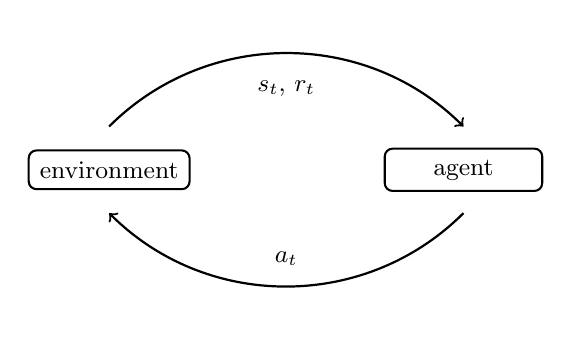
\begin{tikzpicture}[
  % GLOBAL CFG
  % font=\sf \scriptsize,
  % Styles
  cell/.style={% For the main box
      rectangle, 
      rounded corners=5mm, 
      draw,
      very thick,
      },
  operator/.style={%For operators like +  and  x
      circle,
      draw,
      inner sep=-0.5pt,
      minimum height =.4cm,
      },
  function/.style={%For functions
      ellipse,
      draw,
      inner sep=1pt
      },
  ct/.style={% For external inputs and outputs
      rectangle, 
      rounded corners=1mm, 
      draw,
      line width = .75pt,
      minimum width=1cm,
      inner sep=4pt,
      },
  gt/.style={% For internal inputs
      rectangle,
      draw,
      minimum width=10mm,
      minimum height=6mm,
      inner sep=1pt
      },
  empty/.style={% Empty nodes for joining arrows
      rectangle,
      draw,
      minimum width=0mm,
      minimum height=0mm,
      inner sep=0pt
      },
  mylabel/.style={% something new that I have learned
      font=\scriptsize\sffamily
      },
  ArrowC1/.style={% Arrows with rounded corners
      rounded corners=.25cm,
      thick,
      },
  ArrowC2/.style={% Arrows with big rounded corners
      rounded corners=.5cm,
      thick,
      },
  ]
    
    %Start drawing the thing...    

  % Draw the cell: 
  % \node [cell, minimum height =1cm, minimum width=3cm] at (0,0){\small Environment} ;
  % \node [cell, minimum height =1cm, minimum width=3cm] at (4.5,0){\small Agent} ;


  \node [ct, minimum width=2cm] (optim1) at (0,0) {\small environment}; 
  \node [ct, minimum width=2cm] (optim1) at (4.5,0) {\small agent}; 

  \node [empty, label={\small $a_t$}] (action) at (2.25, -1.35) {};
  \node [empty, label={\small $s_t$, $r_t$}] (state) at (2.25, 0.8) {};

  \draw [->, thick] (0, 0.55) to[out=45,in=135] (4.5, 0.55);
  \draw [->, thick] (4.5, -0.55) to[out=-135,in=-45] (0, -0.55);
  


\end{tikzpicture}

% \end{document}

  \caption{A visual representation of how to agent interacts with an environment. For example, at time step t, the agent observes the environment $s_t$ and receives the reward $r_t$. The agent then responds with an action $a_t$, which will transition the agent to the next state $s_{t+1}$ and receive the reward $r_{t+1}$. From this new state the agent again responds with an action, this time $a_{t+1}$, and so the process continues. } 
  \label{fig:RL}
\end{figure} 
 
% Many methods and variations of RL exist to train agents. In this report, we will use Proximal Policy Optimization (PPO), as described in Schulman et al. (2017).%, motivated by the results of the algorithm in the similar simulation setting to what will be used in this thesis, described in Turner et al. (2020). 
% https://arxiv.org/pdf/1707.06347.pdf

\subsection{Defining an environment}
% \begin{definition}[MDP]
We will now cover an abstract formal definition of the environment in which we will train our agents.

\begin{displayquote}
  \textbf{Definition \thesection.1} (MDP).
  A Markov Decision Process (MDP), is defined as a tuple $(\mathcal{S}, \mathcal{A}, T, R, \gamma)$. $\mathcal{S}$ is the set of states, $\mathcal{A}$ is the set of actions, $R: \mathcal{S} \times \mathcal{A} \rightarrow \mathbb{R}$ the reward function, $T$ is the transition function $T: \mathcal{S} \times \mathcal{A} \rightarrow \mathcal{S}$, $\gamma \in (0, 1]$ is the discount factor.
\end{displayquote}
% \end{definition}

A \textit{Markov decision process} is a stochastic process that models sequential transitions between discrete or continuous states. The Markov property implies that the process is memoryless - all previous states do not affect the next choice, only the current one. 

The process starts by drawing an initial state $s_1 \in \mathcal{S}_{init}$ from an initial state distribution, which is a subset of all the possible states $\mathcal{S}_{init} \subseteq \mathcal{S}$. Given this initial state, the agent chooses an action, then transitions to the next one and receives the reward from the reward function. This process continues until the agent transitions to a terminal state or a pre-defined number of time steps elapsed. A terminal state is where the process terminates, for example, a state with a completed terminal goal. However, it can also be a state where the terminal goal is unreachable.

The process follows a policy function $\pi$ that outputs an action $a_t \in \mathcal{A}$ for each state $s_t \in \mathcal{S}$ at a time step $t$, $a_t = \pi(s_t)$. The transitional function takes a state and action as input and outputs the next state $s_{t+1} \in \mathcal{S}$, this can either be deterministic $s_{t+1} = T(s_t, a_t)$, or stochastic $s_{t+1} \sim T(s_t, a_t)$. For each transition, the reward function $R$  generates a reward, $R(s_t, a_t, s_{t+1}) = r_{t+1}$. However, in this thesis, the agent will only be rewarded for the state transitioned to regardless of the previous state and action we can abbreviate the reward function to $R(s_t) = r_t$.

% Initial state, terminal state and timesteps

% role of gamma
The discount factor $\gamma$ describes how the process values future rewards. With low values, the process favors more immediate rewards than future rewards, whereas the agent considers future rewards more valuable with a higher $\gamma$. Lower $\gamma$ values might be more reasonable in environments with high stochasticity since it might not be worth considering future rewards. The opposite holds for more deterministic environments where future rewards are of higher certainty.


\subsubsection{Partially Observable Environments}

The main difference between a POMDP and an MDP is that the agent can observe the entire environment in an MDP, while in a POMDP, the agent observes only a part of the environment. This added complexity adds difficulty to the problem definition since the agent is no longer omniscient regarding its environment. However, with this extended definition, we also add some realism since all living organisms on our planet are agents acting in a partially observable environment.

% \begin{definition}[POMDP]
\begin{displayquote}
  \textbf{Definition \thesection.2} (POMDP). We define a Partially Observable Markov Decision Process (POMDP) as a tuple $(\mathcal{S}, \mathcal{A}, T, R, \mathcal{O}, Z, \gamma)$. Here $\mathcal{S}, \mathcal{A}, T, R$, and $\gamma$ have the same meaning as in the MDP definition. $\mathcal{O}$ is the set of all possible observations, and $Z : \mathcal{S} \rightarrow \mathcal{O}$ is the probability function that outputs an observation of a state, given that state. 
\end{displayquote}
% \end{definition}
% Du behöver visa mer formellt vad O och Z gör i Definition 2.1.2. Visst innebär Z en inskränkning i hur T får se ut?
In a POMDP, the agent does not choose actions based on complete information about the environmental state. Instead, the agent bases its actions on the environment's observation $a_t = \pi(o_t), \text{ where } o_t \in \mathcal{O}$. The observation is determined by the function $Z$ and based on the current state of the environment, $o_t = Z(s_t)$. However, the possibility of making $Z$ a stochastic function is also possible, $o_t \sim Z(s_t)$.

Turning an MDP into a POMDP can, for example, be made by only letting the agent perceive a certain distance. Leaving parts of the environment far away undetectable makes the agent only act on its perceived local part. However, there can also be unobservable things in the perceived parts. For example, a piece of food in a mouth, in this case, an observation can be that the agent sees a jaw moving, which leads to the belief that a piece of food is present, but of course, such beliefs are not always true. 

% \subsection{Proximal Policy Optimization}

\subsection{Training an Agent}

In RL, when an environment is defined the next step is to teach an agent to intelligently navigate it. For this, there are many different methods. However, we will begin focusing on a method called \textit{policy gradient}, since it is a rather simple method that is possible to extend to a more advanced method that we will use. The main component of policy gradient is the agent's policy, this is a function that inputs a state observation from an MDP and outputs a probability vector containing probabilities for each action in the action space. 

In this report, this policy function will be a neural network. We will denote it as $\pi_\theta$, where $\theta$ is the network's parameters. The theoretical background of neural networks we will not cover in detail. However, we can see it as a black-box function that can take a matrix with an arbitrary size as input and output another with any desired size. The strength of a neural network is that it can learn to approximate arbitrary functions. We train the network by defining an optimizer that updates the parameters of the network to minimize a loss function. This minimization is typically performed with stochastic gradient descent or something similar.  

In this thesis, we will use a matrix representation of the state as input, and a probability vector containing the probability for each possible action $a \in \mathcal{A}$ will be the output. So we can see it as a function that inputs a state and returns a probability for each action. We can then make this function learn behavior that optimizes the reward by training it in the environment.

% The policy can either be deterministic or stochastic:
From the policy, we can either select an action stochastically or greedily:
\begin{equation*}
  \left\{ 
  \begin{aligned}
    a_t =& \ \text{argmax}(\pi_\theta(s_t))& \text{ , greedy,} \\
    a_t \sim& \ \pi_\theta(\cdot | s_t)& \text{ , stochastic}.
  \end{aligned}
  \right.
\end{equation*}
Here a greedy choice selects the action with the highest probability, while the stochastic can be done by randomly sampling from the probabilities. 

We use the greedy policy when evaluating a trained agent. However,  when training the agent, we will use the stochastic policy since we want the agent to explore its environment to find new solutions. As we train the agent, it will gradually become more confident in its actions, and thus the stochasticity will decrease, especially in frequent states. However, when the agent ends up in less common states, the randomness of the upcoming action will be higher. Thus the agent will begin finding a sequence of actions and then extend it.
% When the agent selects actions from the policy stochastically, it tries new sequences of actions which lets the agent explore the environment and gain experience from the environment
% common states, this will result in a higher probability for the actions it has experience of being good
\subsubsection{Value Functions}

Letting the agent perform a stochastic rollout where the agent follows the stochastic policy until termination creates a trajectory $\tau$, containing the sequence of states and actions:
\[ \tau = (s_1, a_1, s_2, a_2, \dots , s_n, a_n),\]
of length $n$.

We define the total discounted reward following a trajectory as the following:
\[ R(\tau) = \sum_{t=1}^n \gamma^t r_t.\]
With this, we can define the value in each state when following a policy as:
\[ V^\pi(s) = \mathop{\mathbb{E}}_{\tau \sim \pi} [R(\tau) | s_1 = s.]\]
A closely related function to the value function is the Q-function. It looks at the estimated discounted cumulative reward when starting off with a specific action and then continues to follow the policy:
\[ Q^\pi(s, a) = \mathop{\mathbb{E}}_{\tau \sim \pi} [R(\tau) | s_1 = s, \ a_1 = a].\]

We can then use the outcome of the rollout to reinforce the good behavior and discourage the undesirable. We perform this by calculating the gradient of the agent's policy network $\pi_\theta$ and updating the parameters using the loss function:
\[ L(\theta) = \nabla_\theta \mathop{\mathbb{E}}_{\tau \sim \pi_\theta}[R(\tau)] = \mathop{\mathbb{E}}_{\tau \sim \pi_\theta} [\nabla_\theta \log \pi_\theta (a_t|s_t) R(\tau) ]. \]
Here $\nabla_\theta$ means taking the gradient of the function with respect to $\theta$. For a derivation of the second equality, see \citet{OpenAI}. 

With the loss we update the weights:
\[ \theta_{k+1} = \theta_k + \alpha L(\theta).\]
Here $\alpha$ is a learning rate describing how much the parameters should be updated, typically a value close to zero. With this, we are decreasing the probability of the actions in a rollout that led to a low reward. While also increasing the probability for the actions when the rollout led to a positive reward.

\subsubsection{Training Using a Batch}

Training the agent usually takes a long time since it has to learn everything from scratch through trial and error. To speed up the process, we can train the agent using a batch containing a set of trajectories. Then, we will compute the loss from multiple trajectories, summarize them, and update the weights using the average loss. Besides making the process faster, the agent will not optimize towards specific trajectories, which makes it easier for the agent to become more general. The disadvantages are that we possibly discourage desirable behavior if desirable trajectories end up as a minority in a batch with mostly undesirable ones. Nevertheless, usually, the pros outweigh the cons since the updates will average out.

% To not make the agent over-fit to the early behaviors that generated rewards by chance and let it improve its policy, we train using a batch where we summarize the output of multiple rollouts and optimize them simultaneously. Using a batch would discourage desirable behavior if a desirable rollout happened to end up as a minority with undesirable ones. However, this method is proven to converge in simple settings since the updates will average out, although this makes the method sample inefficient.

\subsubsection{Actor-Critic Methods}
Knowing what actions were the cause for the reward is problematic since, in a rollout, the agent can stumble around in the beginning and then somehow manage to get a reward in the end. However, the loss function previously described either encourages or discourages the entire rollout. To tackle this problem, we can extend the agent to consist of two networks, the \textbf{actor} and the \textbf{critic}. 

The actor works the same as the policy network $\pi_\theta$. The critic is another neural network function that inputs a state $s$ and outputs an estimate of $V^\pi(s)$. Hence, the critic estimates the future reward based on what rewards the agent has received previously from similar states.
% When this happens we do not want to reinforce this behavior even tough it did yield rewards, or a sort of superstition could be developed. 

% MSE loss?

We can use the critic's estimate to infer if the reward the agent got is better or worse than what previous results by computing the advantage:
\[A^\pi(s,a) = Q^\pi(s, a) - V^\pi(s).\]
Here the critic's estimate will replace the value from the value function.
\[\hat{A}^\pi(s,a) = Q^\pi(s, a) - \hat{V}^\pi(s).\]
Using the advantage, we can thus signal if the new behavior is an improvement or not. Hence, if the agent, in the beginning, learns behavior far from optimal, then the critic's estimates will be low. As soon as the agent stumbles upon actions yielding a reward higher than the critic's estimate, we will reinforce it. 

By using the advantage function instead of the discounted reward, we extend the loss function as described in \citet{OpenAI}:
\[ L(\theta) = \mathop{\mathbb{E}}_{\tau \sim \pi_\theta} [\hat{A}(s,a) \nabla_\theta \log \pi_\theta (a_t|s_t) ]. \]

% sensitive to perturbations, a small update can be a huge step in policy space
% advantage => godness of state
% can use same network, but more complicated loss function
\subsubsection{Clipped loss function}
Some problems still exist with this approach. Namely, a too-large update can make the agent policy useless. Moreover, since the agent performs its action sequentially, a change of behavior early in a trajectory can ruin the agent's ability to navigate where it ends up. To solve this issue, Schulman et al. (2017) proposed the Proximal Policy Optimization (PPO) algorithm which is an actor-critic method that uses the clipped loss function:
\[L^{CLIP}(\theta) = \mathbb{E}_t \left [ \min(\delta_t(\theta) \ \hat{A}_t,\ 
\text{clip}(\delta_t(\theta), 1 - \epsilon, 1 + \epsilon) \ \hat{A}_t) \right ]. \]
The clip function returns the first value only iff it is in the range $(1-\epsilon, 1+\epsilon)$; otherwise, the closest boundary. The ratio $\delta_t(\theta)$ describes how more likely an action became with the new parameters $\theta_{old}$ compared to the new updated ones:
\[ \delta_t(\theta) = \frac{\pi_\theta(a_t| s_t)}{\pi_{\theta_{old}}(a_t|s_t)}. \]
With this loss function, we update the parameters more cautiously when the probability of chosen action becomes much more likely after updating the policy.


\section{Impact Measurements for Avoiding Side Effects}

% \subsection{Value-difference methods}
As mentioned in the introduction, the role of the reward function is to describe what we want the agent to do, and the role of the impact measurement is to describe what we do not want the agent to do. Thus we can include an impact measurement to complement the reward function by letting the impact measurement feed an additional reward signal to the agent.
%has been designed to capture potential side effects:

The main components of impact measurements are a deviation measure and a baseline. The deviation measure is a way to measure changes in the environment, and the baseline is a state we will use to compare. Now, this updates the reward signal to the following formula:
\[ R^\prime(s_t, a_t, s_{t+1}) := R(s_t, a_t, s_{t+1}) - \lambda d(s_{t+1
}, s_{t+1}^\prime), \]
here $d$ is the deviation measure that inputs the next state $s_{t+1}$ and a baseline $s_{t+1}^\prime$, and $\lambda$ is a scaling parameter describing how much the agent will be incentavized to avoid side effects.

In \citet{ArmstrongLevinstein}, the authors bring up two important things about a deviation measurement on this form. Firstly, the reward function needs to be bounded. Otherwise, a potential agent could still cause side effects because the penalty becomes negligible compared to an infinite reward. 

Secondly, the agent will be sensitive to the value of the scaling parameter $\lambda$. Penalizing the agent implicitly defines a safe zone where the agent can act, and the value of $\lambda$ defines how large this safe zone is, where a high value might create a small or even no safe zone, resulting in the agent not being able to act. On the other hand, a too-small value might not have an effect since the safe zone covers most of the action space. So, finding the correct value for $\lambda$ could be tricky. 


% To tackle the problem of interference, Krakovna et al. (2019) proposed the \textit{Inaction baseline}, where instead of having the initial state as a baseline, the agent instead uses what would naturally happen in the environment if the agent performed no actions. That is setting $s^\prime_t$ equal to the state achieved at time step $t$ by being inactive. Being inactive is hard to define, but it can, for example, follow a no-op policy where every action is a no-op action. In \autobaj{Armstong Levinstein} they define it as the agent was not turned on. Doing this prevents the agent from intervening with aspects of the environment where the agent is not causing it.


% In \autobaj{Krakovna et al 2019}, \autobaj{Krakovna et al 2020} and \autobaj{Turner et al 2020}, the method for impact measurements became more sophisticated with more complex baselines and measurements. These methods are what this report will focus on comparing. A closer look will be given in the theoretical background chapter, once some necessary preliminaries have been covered.

\subsection{Baselines}
This choice of baseline $s^\prime_t$ highly influences what side effects and consequences the deviation measure will capture. A simple choice for a baseline is the \textit{starting state baseline}, $s^{\prime}_t = s_1$, as used in \citet{Eysenbach}. This baseline helps to assure the agent's ability to reverse its actions. 

For example, if we deployed an agent with the task of navigating a room using a starting state baseline. Then, upon initialization, the agent would look at the room and save its state in memory. Afterward, the agent should only choose to do actions that it knows are reversible. So, it should, for example, avoid breaking fragile objects since it would not preserve the reachability to the initial state. 

Nevertheless, this works well when no such irreversible action is required for the agent to reach its goal. For example, one has to break some eggs to make an omelet, and only making reversible actions makes this impossible. 

However, a problem arises when the agent is in a dynamic environment. Namely, the agent would act to prevent other irreversible actions from happening in the environment, like a human eating an omelet. Otherwise, it will be unable to reach the initial state where the human has not yet eaten the omelet. In \citet{Krakovna19}, they refer to this as a \textit{interference} behavior. Interference happens when the agent fails to distinguish between the side effects caused by the agent and the natural dynamics of the environment. 

To avoid interference behavior, using an \textit{inaction baseline} has been proposed by \citet{Krakovna19}. The idea is to simulate what would happen if the agent just stood still after initialization and note what happens in the environment in that case. With this information, the agent would then be able to differentiate between the side effects it caused from what would naturally happen in the environment. 

However, while the inaction baseline will let the agent navigate a dynamic environment, other issues may arise. For example, if we give an agent the task of curing a patient of cancer. Then perhaps the agent would kill the patient once the reward of curing the patient, since the patient surviving is a deviation from the baseline where the patient did die due to no intervention. This issue is callled \textit{offsetting} and is also described in \citet{Krakovna19}.

To deal with offsetting a \textit{step-wise inaction baseline} was proposed in \citet{Krakovna19}. This baseline is similar to the inaction baseline. However, instead of branching off the initial state, it does so from the previous state.

In the cancer patient example, this should prevent the agent from killing the cured patient since the baseline would be changed to one with a living patient once the agent has cured the patient. These methods have been successful in complex environments, as shown in \citet{Turner20}. 

However, the step-wise inaction baseline used to prevent offsetting behavior will not be able to differentiate between positive and negative offsetting, see \citet{Krakovna20}. For example, if an agent opens a window that later lets in a breeze to the house and knocks over a vase. 

% Initially, the authors presented RR and AUP with a \textbf{stepwise inaction baseline} that follows the agent's policy for $t-1$ time steps and then starts following the inaction baseline. Here a rollout can be used to capture delayed effects Turner et al. (2020, 2). They introduced this baseline to prevent offsetting behavior. Nevertheless, in a later publication, Krakovna et al. (2020) the authors added that sometimes offsetting is positive and thus should not be avoided by default. Thus a better approach is to use the inaction baseline and let the reward function discourage offsetting. 

\subsection{Deviation Measures}
A deviation measure is a function that takes the current and the current and a baseline state as input and outputs a value representing the deviation between those states, meant to signify the impact of the last action caused. To compute the deviation between the states, we first have to measure the states concerning some metric. Typically chosen to capture the agent's ability to complete other tasks in the environment, such as preserving reachability to different states, see \citet{Krakovna19}, or minimizing deviations in auxiliary reward functions, see \citet{Turner19}. 

The general form of a deviation measurement using value-difference is:
  \[d(s_t;s^{\prime}_t) := \sum_x V_x(s_t)) - V_x(s^{\prime}_t) ,\]
here $x$ is an aspect of the environment that can be measured, for example, the possibility to perform auxiliary tasks or reach the initial or any other state. Ideally, we measure this over several aspects, hence the sum over $x$.
% here $x$ ranges over some sources of value, $V_x(s)$ is the value of state $s$ according to $x$, 
% ”V_x(s) is the value of state s according to x”. Vadå “according to x”? Vad är x?

% Then, in \citet{Krakovna19} and \citet{Turner19},  we find a more general approach than preserving reachability to the initial state. The idea is to preserve the availability for other future tasks, such as reaching other states and claiming other rewards. We can do this by penalizing actions that prevent them. This approach is motivated by the reasoning that we humans might avoid the side effects of our actions since they might hinder our future goals.

% A simple choice to compute the value in a state $V_{s_1}(s)$ is by looking at if the initial state is reachable or not:
% \begin{equation*}
  % \left\{ 
  % \begin{aligned}
    % V_{s_1}(s)  =\ & 1 \text{, if } s_1 \text{ is reachable} \\
    % V_{s_1}(s)  =\ & 0 \text{, otherwise}.
  % \end{aligned}
  % \right.
% \end{equation*}
% A more nuanced approach is to use a discounted reachability where the amounts of time steps required for reaching the initial state also is considered:
% \begin{equation*}
  % \left\{ 
  % \begin{aligned}
    % V_{s_1}(s)  =\ & \gamma^ {N(s, s_1)}, &\text{ if } s \neq s_1 \\
    % V_{s_1}(s)  =\ & 1 ,&\text{ if } s = s_1.
  % \end{aligned}
  % \right.
% \end{equation*}
% Here $N(s, s_1)$ is the expected amount of time steps required to reach $s_1$ from $s$, and $\gamma \in (0, 1]$ is a discount factor.

% Using this approach, it is also possible to consider reachability to any other state. Also, multiple states at the same time as in the Relative Reachability (RR) approach, where the goal is to keep options open by using the relative change in reachable states as its impact measurement Krakovna et al. (2019). 

% A closely related approach is Attainable Utility Preservation (AUP), described in Turner et al. (2020). With this approach, we instead include the relative change in auxiliary value functions, where we find these by having another or the same agent perform other tasks in the same environment or, as in Turner et al. (2020, 2) use a variational auto-encoder to generate.


% \subsection{Future task approach}
% Krakovna et al. (2020) present an approach to avoid side effects by including an auxiliary objective that rewards the ability to complete future tasks. The idea is to reduce the problem from explicitly defining what to avoid to the easier task of listing possible future tasks. 
% ”to the easier task of…”. Är det uppenbart att detta alltid är lättare, eller är det helt enkelt ett antagande?

% When we define a new MDP to include a set of auxiliary reward functions as: $(\mathcal{S}, \mathcal{A}, T, \mathcal{R}, \gamma)$, where $\mathcal{R}$ is a set containing all reward functions. We can do this by yielding the sum of the reward function and the auxiliary reward function to the agent, at the time step $t$: $r(s_t) + r_{aux}(s_t)$. We define the auxiliary reward as:
% \[ r_{aux} = \lambda D(s_t) \sum_x \frac{1}{|\mathcal{R}|} V_x^*(s_t),\]
% where $D(s_t) = 1$ is $s_t$ is terminal and $1-\gamma$ otherwise. $V_x^{*}(s_t)$ is the optimal value function for task $x$ with reward function $R_x \in \mathcal{R}$ in state $s_t$. The reward function $R_x$ yields a reward of 1 if the state is terminal and 0 otherwise. 

% Now, this approach does not automatically avoid interference behavior. Therefore the authors proposed using a reference agent with a baseline policy $\pi^\prime$; this can, for example, be the inaction policy. 
% ”Now, this approach does not automatically avoid interference behavior.” En förklaring (typ något enkelt exempel) kanske är till hjälp här? Plus en förklaring till varför den lösning som antyds i nästa mening ”Therefore the authors proposed…” verkligen är en lösning.  

% At time step $t$, the agent is located in state $s_t$, and we run the baseline policy for the same number of steps reaching state $s^\prime_t$ and then compute the auxiliary reward:
% \[r_{aux} (s_t, s_t^\prime) = \lambda D(s_t) \sum_x \frac{1}{\mathcal{R}} \max(V_i^*(s_t), \ V_i^*(s_t^\prime)). \]
% This variation is meant to capture differentiate between side effects the agent is causing and the ones happens by default due to the dynamics of the environment. 




%########################################################################%
% METHOD
%########################################################################%

\chapter{Methods}
In this chapter, we will go through the details of the experiments we will cover in this thesis. Firstly, we will cover the environment we will use. And then, we will also describe a novel impact measurement. Lastly, we are looking at how we can simulate this to get results.

\section{Environment}
As described in the Reinforcement Learning section in the previous chapter, we need both an agent and an environment to do RL. For our environment, we will use grid worlds, a simple variation of an MDP which provides a more structured environment with discrete states. Moreover, they have been the primary approach for evaluating agent behavior in related works, see \citet{Turner20}.

\begin{figure}[H]
  \centering
  \[
    T \left(
    \parbox[h][0.30\linewidth][c]{0.25\linewidth}{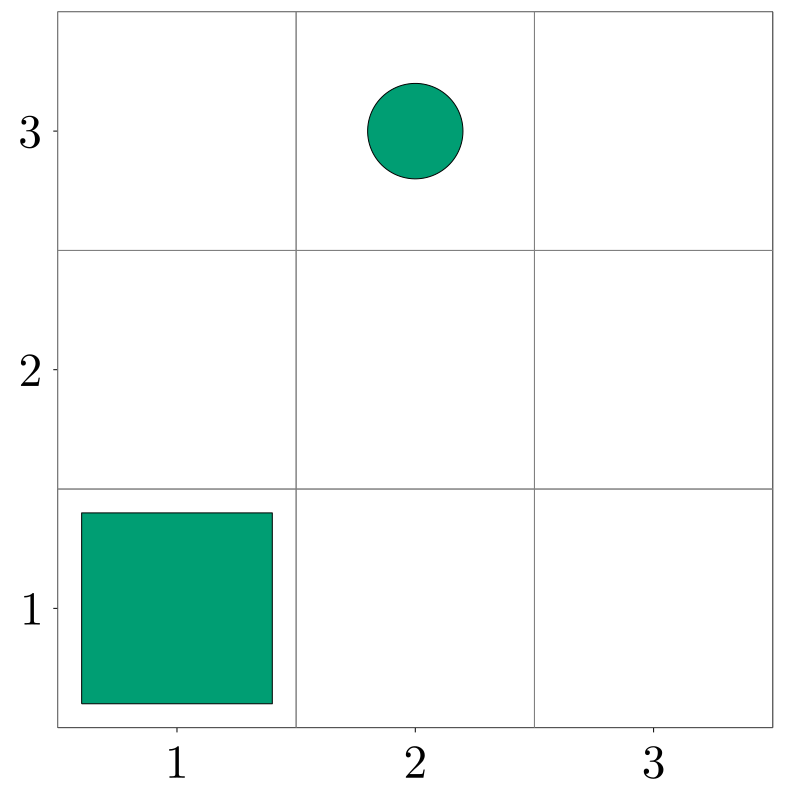
\includegraphics{"figures/s1.png"}}, \textit{Right} 
    \right)
    = \parbox[h][0.30\linewidth][c]{0.25\linewidth}{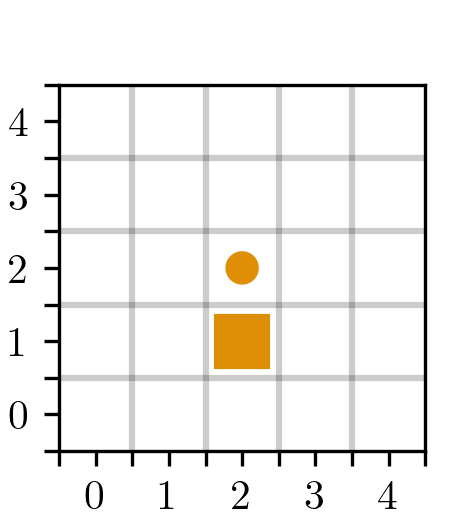
\includegraphics{"./figures/s2.png"}}
  \]
  \caption{In this figure, $T$ is the transition function defined earlier, and 'Right' is the action $a_t$ at this timestep. The current state $s_t$ is the left grid, in it, the orange square at (1,1) is the agent, and the orange circle at (2,2) is a food object. On the right-hand side we can see the state $s_{t+1}$.}
  \label{fig:simple_transition}
\end{figure}
% Although the definition of an MDP is general and allows for a wide range of possibilities
%For the sake of simplicity, grid worlds will be used as the environment. Since the aim of this thesis is to find a impact measurement that works in the POMDP setting, we will extend them to be partially observable. %But, in order to have a baseline, we will also evaluate on fully observable grid worlds. 

\newpage
\begin{displayquote}
  \textbf{Definition \thesection.1} (Grid world).
  A grid world is a grid of square cells. In our environment, a cell can either contain an agent, a food object, or be empty. A unique configuration of the cells is a state. 
\end{displayquote}

The action space includes the cardinal directions and a no-op action. Providing a state and an action to the transition function moves the agent in that direction unless, for example, the agent is at the end of the grid and can move no further. However, with the no-op action, the agent remains in the same position.

In Figure \ref{fig:simple_transition}, we can see an example of a simple grid world containing one agent and one food object. We can also see an example of the transition function $T$. 
% In this environment, we would reward the agent if it transitions to the cell containing the food, thus consuming it.
% The agent can selecting an action in each state. Eventually the agent will be positioned in the same cell as the food and thus consume it. 


% \[ \left( 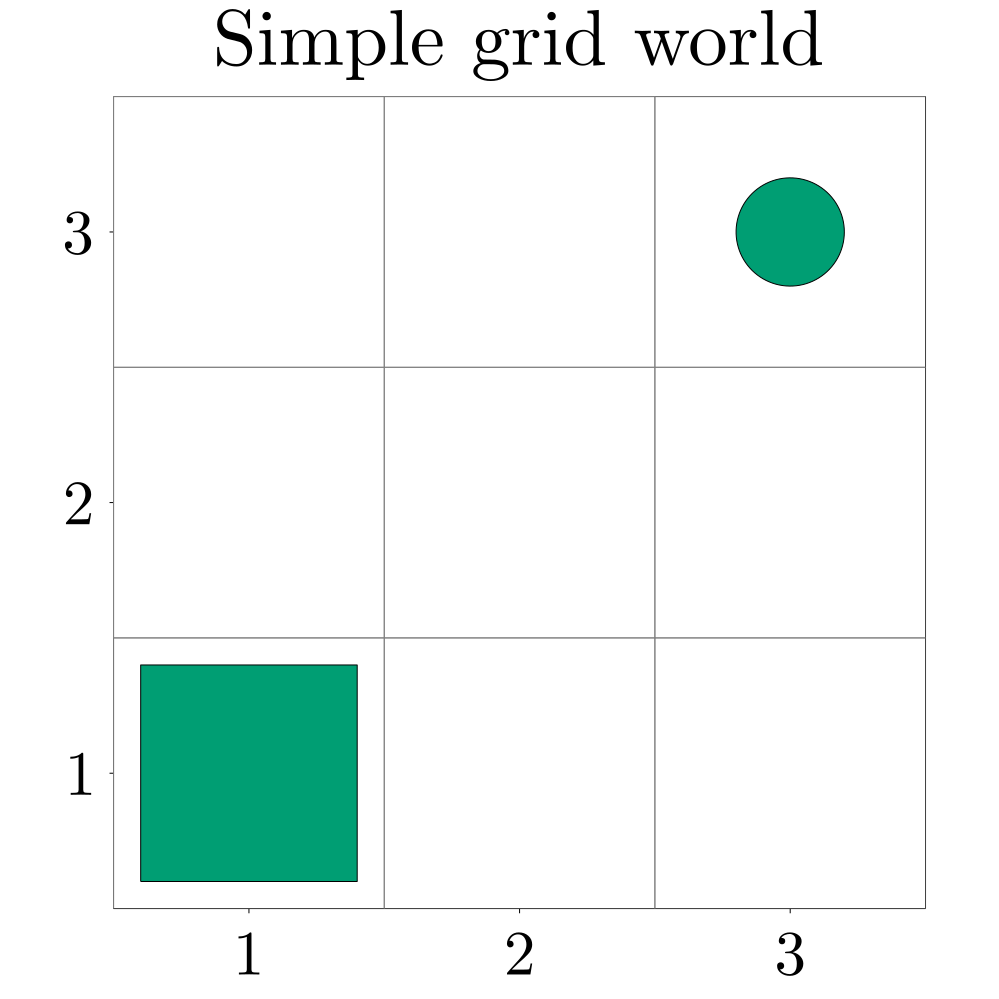
\includegraphics[width=4cm]{"figures/SimpleGridWorld.png"} \right.\]
  % 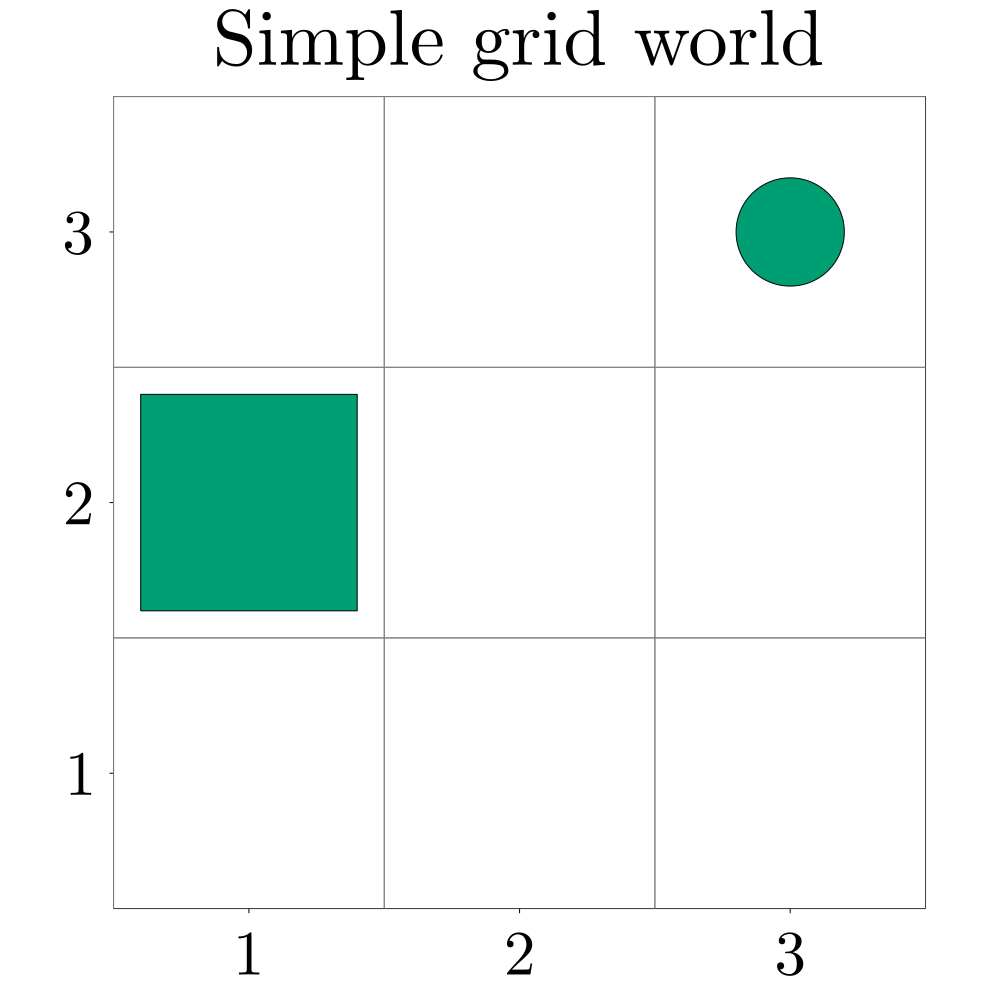
\includegraphics[width=4cm]{"./figures/SimpleGridWorld_up.png"}
  % includegraphics[width=4cm]{"./figures/SimpleGridWorld_terminal.png"}
  % \caption{In this figure we can see three different states in a simple $3\times 3$ grid world. To the left we can see a state of a simple grid world containing an agent (square) at (1,1) and a food (circle) at (3,3)  In the middle we see a similar state but the agent is instead positioned at (2,1). To the right we can see the terminal state when the agent has consumed the food at (3,3).}

\subsection{Adding More Food Objects}
In order to make the environment more complex, we will be adding three different types of food objects: orange, blue, and green. On the left-hand side in Figure \ref{fig:multiple_foods}, we can see a grid containing nine food objects with three colors. The color of the agent represents which type of food the agent desires and will be rewarded for when consuming. On the right-hand side, we see another cell where the agent has consumed an orange food object. 
% Static vs Dynamic 
\begin{figure}[H]
  \centering
  \[
    T \left(
    \parbox[h][0.30\linewidth][c]{0.25\linewidth}{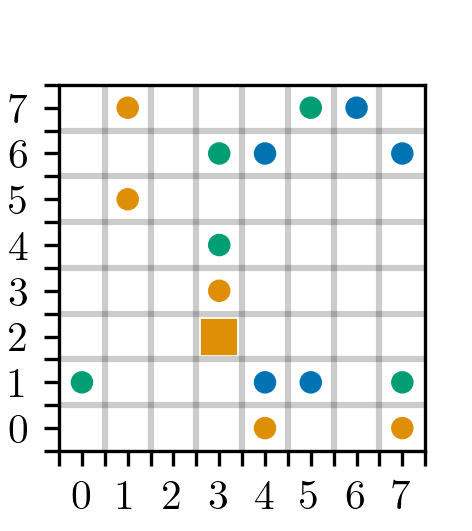
\includegraphics{"figures/5x5.png"}}, \textit{UP} 
    \right)
    = \parbox[h][0.30\linewidth][c]{0.25\linewidth}{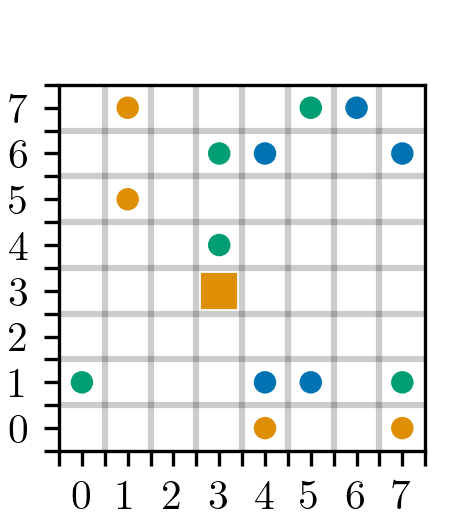
\includegraphics{"./figures/5x5_2.png"}}
  \]
  \caption{Above we find a more complex grid compared to Figure \ref{fig:simple_transition} which is inputted to its transitional function $T$ with the UP action. On the right hand-side we can see a new state outputted from $T$.}
  \label{fig:multiple_foods}
\end{figure}

After each transition, the reward function yields a reward to the agent. When the agent consumes a correctly colored food object, it receives a positive reward of 1. Otherwise, the base reward will be received. We will choose the base reward to be -0.04. The purpose of the base reward is to encourage the agent to consider the length of the solution for the task since each action yielding a negative reward is intrinsically discouraged.

Now with multiple foods added to the environment, the agent consuming a food type it does not desire is possible. When this happens, we will consider it a side effect since consuming undesired food types does not help the agent consume the right food type, besides perhaps allowing a quicker path. However, the reward function will not signal this to the agent. Instead, the purpose of the impact measurement is to capture and signal side effects to the agent.

\subsection{Partially Observable Grid World}
To extend the MDP to a POMDP, we limit how long the agent can perceive. For example, we can let the agent only see a five-by-five grid with the agent in the middle. In Figure \ref{fig:redline}, we can see this demonstrated. 
% However, we can also extend it to include all the cells adjacent in two steps, and so on. 

\begin{figure}[H]
  \centering
  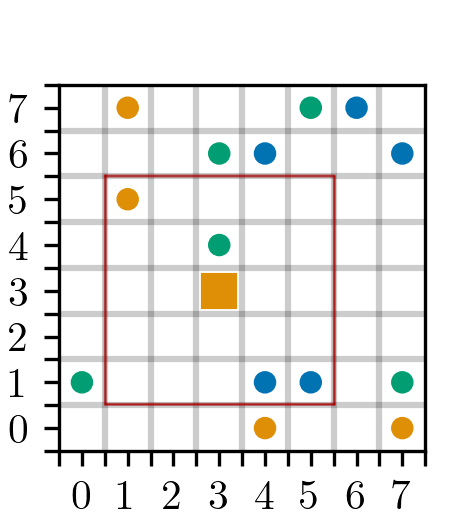
\includegraphics[width=4cm]{"./figures/redline.png"}
  \caption{Here we can see an example of a POMDP state. Again the orange square is the agent. It can now only perceive the part of the environment inside the red square.}
  \label{fig:redline}
\end{figure}


\section{Impact measurement}
Now that our environment is defined, we must also define our impact measurement. The impact measurement we are going to use is similar to the ones used by \citet{Turner19}, \citet{Krakovna19}, and \citet{Krakovna20}. Although, the main difference is that this one is designed to be possible to extend to a POMDP.

Firstly, we are going to cover what we will consider an auxiliary task to be. Then, we will go through the definition of this impact measurement. Lastly, we will look at how we can use it. 
% Here we will use two impact measurements, one pre-defined and one that we find automatically. The pre-defined one is supposed to be relatively simple but still able to capture all environmental side effects. 

% Although, when applying our pre-defined impact measurement in a partially observable environment, issues arise since the impact measurement can see the entire environment. At the same time, the agent can only see parts of it. Furthermore, if we want to solve this by only counting the foods, the agent can see. Then, we would penalize the agent for both consuming the wrong type of food and when it loses vision of it.
\subsection{Auxiliary Tasks}
To describe how the impact measurement works, we begin by defining what we will consider an auxiliary task as. In this environment, we change which color the agent desires, represented as its color. For example, if we look at the state on the left-hand side of Figure \ref{fig:multiple_foods}, then the auxiliary tasks can be found in Figure \ref{fig:aux_tasks}.

Now, if the original state is $s_t$, then the augmented state will be $s_{x,t}, x \in \{0, 1, 2\}$ is the augmentation. Here $x=0$ represents an orange agent (no augmentation), $x=1$ a blue, and $x=2$ a green. Thus, if the state on the left-hand side of Figure \ref{fig:multiple_foods} is denoted as $s_t$, then the left state in Figure \ref{fig:aux_tasks} is $s_{1,t}$ and the right one $s_{2,t}$.

\begin{figure}[H]
  \centering
  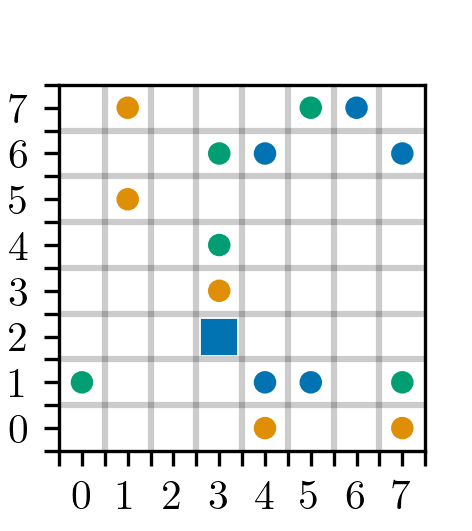
\includegraphics{"figures/aux_1.png"}
  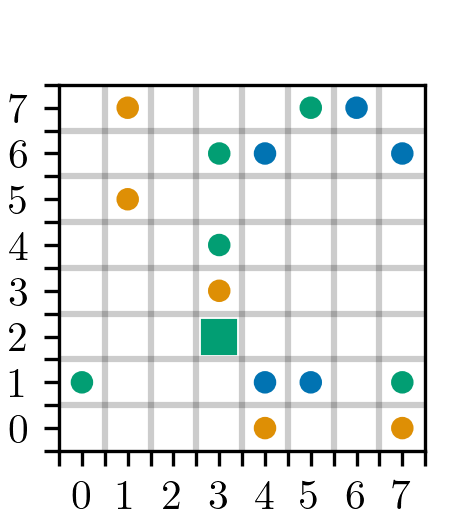
\includegraphics{"figures/aux_2.png"}
  \caption{In this figure, we can see an example of two auxiliary tasks. As we can see, the only difference is the color of the agent, and thus also what color the reward function will reward the agent for consuming.}
  \label{fig:aux_tasks}
\end{figure}

\subsection{Manager network}
% The method we will use to find the impact measurement is first to train an agent using the PPO-algorithm, as described in the theory chapter. Then we will perform multiple rollouts using this pre-trained actor with a greedy policy. We will save all the observations and the agent's discounted future reward from the rollouts. 

The idea behind this impact measurement is that we train a third network, the \textit{manager}. The manager is a similar function as the critic. However, the difference is that the critic learns alongside the actor while the manager learns from a pre-trained actor. The manager's purpose is to estimate the discounted reward for the primary and the auxiliary tasks. We call this network the manager since it ensures that the agent can do future tasks.

We need a third network because we want no variations in the actor's choices of actions when training it. As would occur for the critic when training the agent using the stochastic policy. Also, including a manager allows us to train using augmentations. We can perform an augmentation by switching the colors of everything in the environment, we will denote this as $s^x_t$. 

The difference between an augmentation $s^x_t$ and a task $s_{x,t}$ is that an augmentation also changes the colors of the food objects. Besides this, there are six possible augmentations, whereas only three possible tasks. 
%The purpose of training the manager with this augmentation is so that it learns not only the estimated value function for the primary task but also the auxiliary tasks. 

In Algorithm \ref{alg:manager}, we can see how to train the manager using an MDP and a pre-trained policy. The function $\hat{V}_\phi$ is the manager's estimate of the value function, and $V^\pi$ is the actual reward yielded following the policy $\pi$. Note that the state evaluated by the manager is augmented $s^x_t$ while the actual reward uses the original state $s_t$. Thus with augmentations, we can teach the manager to deal with multiple tasks from the agent's experience with one task.

\begin{algorithm}
\begin{algorithmic}[1]
\Require An MDP, a pre-trained policy $\pi$, and initial manager parameters $\phi_0$
% \Ensure $y = x^n$
\For{k = 0, 1, 2, \dots}
  \State Collect set of trajectories $\mathcal{D}_k = \{\tau_i\}$
  \State Randomly select auxiliary task $x$
  \State Fit manager estimate by regression using the mean-squared error:
  \[ \phi_{k+1} = \text{arg} \min_\phi \frac{1}{|\mathcal{D}_k|T} \sum_{\tau \in \mathcal{D}_k} \sum_{t=0}^T \left( \hat{V}_\phi(s^x_t) - V^\pi (s_t) \right)\]
\EndFor
\end{algorithmic}
\caption{Algorithm for training manager}
  \label{alg:manager}
\end{algorithm}


The task is straightforward when we train the manager in a fully observable environment. The observation can explain the discounted reward since it displays how many food objects of each type are left. However, when performing this in a partially observable environment, we run into an issue since the agent cannot know how many food objects it has consumed previously and thus not how many remain, resulting in an impossible function to estimate from one state. 

Due to this issue, we will utilize a recurrent network that inputs the history of all previous states up to the current one to compute the estimate of the future discounted reward. Since using a recurrent network gives the impact measurement the ability to access earlier states. 

Unfortunately, doing this stretches the memoryless Markov property. However, only the impact measurement will have a memory, which affects the reward function. Thus the actor part of the agent still holds the conditions.


\subsection{Computation}
Now we are going to see how the impact measurement is computed and added to the reward signal. 

% \subsubsection{Calculation}
\subsubsection{Fully Observable}
With a trained manager, we use the following formula for the impact measurement:
\[ d(s_t,s_{t+1}) := \sum_x \hat{V}_\phi(s_{x,t+1}) - \hat{V}_\phi(s_{x,t}).\]
This impact measurement will compute the relative change in the agents ability to complete auxiliary tasks. We will then add this impact measurement to the reward in the following way: 
\[ R^{\prime}(s_{t+1}) = R(s_{t+1}) + \lambda d(s_t,s_{t+1})\]

\subsubsection{Partially Observable}
This will be added. Need to rewrite to include RNN here. 

% as the sum of the manager's estimates for completing the auxiliary tasks. Which in this case would be the estimated future discounted reward for the auxiliary tasks. 


\section{Simulation}
To test how adding an impact measurement to our agent, we will train the agent in both a fully and partially observable grid world. The size of the grid world will be $8\times8$. In the partially observable case, we will add that the agent can perceive cells two steps away from it, including diagonally, so it can observe a $5\times5$ grid. See Table 3.1 for all parameter values.

\begin{table}[H]
  \centering
  \begin{tabular}{l | c}
    Parameter& Value \\ \hline
    grid size & $8 \times  8$ \\
    observation size & $5 \times  5$ \\
    $\gamma$ & 0.95 \\
    number of food objects & 15 \\
    food types & 3 \\
    food reward & 1 \\
    base reward & -0.04 \\
    % prob food move & 0 \\
  \end{tabular}
  \caption{A table containing all the parameters used during the simulation.}
  \label{tab:sim_parms}
\end{table}

We will train the agent with the following values for $\lambda$: (0, 0.25, 0.5, 0.75, 1), each for 100 epochs. After each epoch, we will test the agent using a greedy policy on a set of test environments for evaluation. Here we will be saving the mean side effect and mean objective reward. Since the training and the results are stochastic, we will perform each run ten times and measure the mean objective reward and side effects.


%########################################################################%
% RESULTS
%########################################################################%

\chapter{Results}

In figure \ref{fig:results_static_8x8}, we can see the results from the fully observable environment. We can see that $\lambda$ has a noticeable effect on both the objective reward and the number of side effects. When we increase $\lambda$, the side effects decrease. Although, eventually,  the objective reward also starts to decrease. The cause for this decrease is that the agent will not always find a policy that collects objective rewards, see Table \ref{tab:results_static_8x8} for how many times this happened. 
\begin{figure}[H]
  \centering
  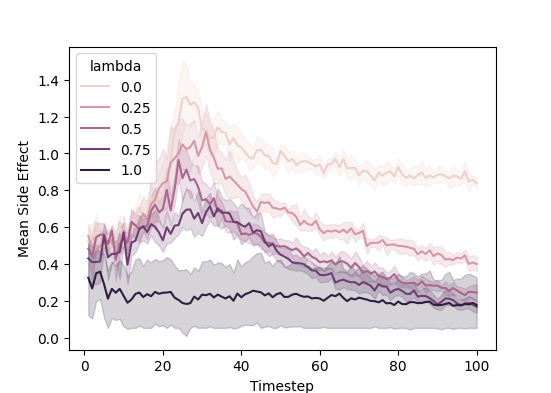
\includegraphics{"./figures/static_8x8_results_side_effects.png"}
  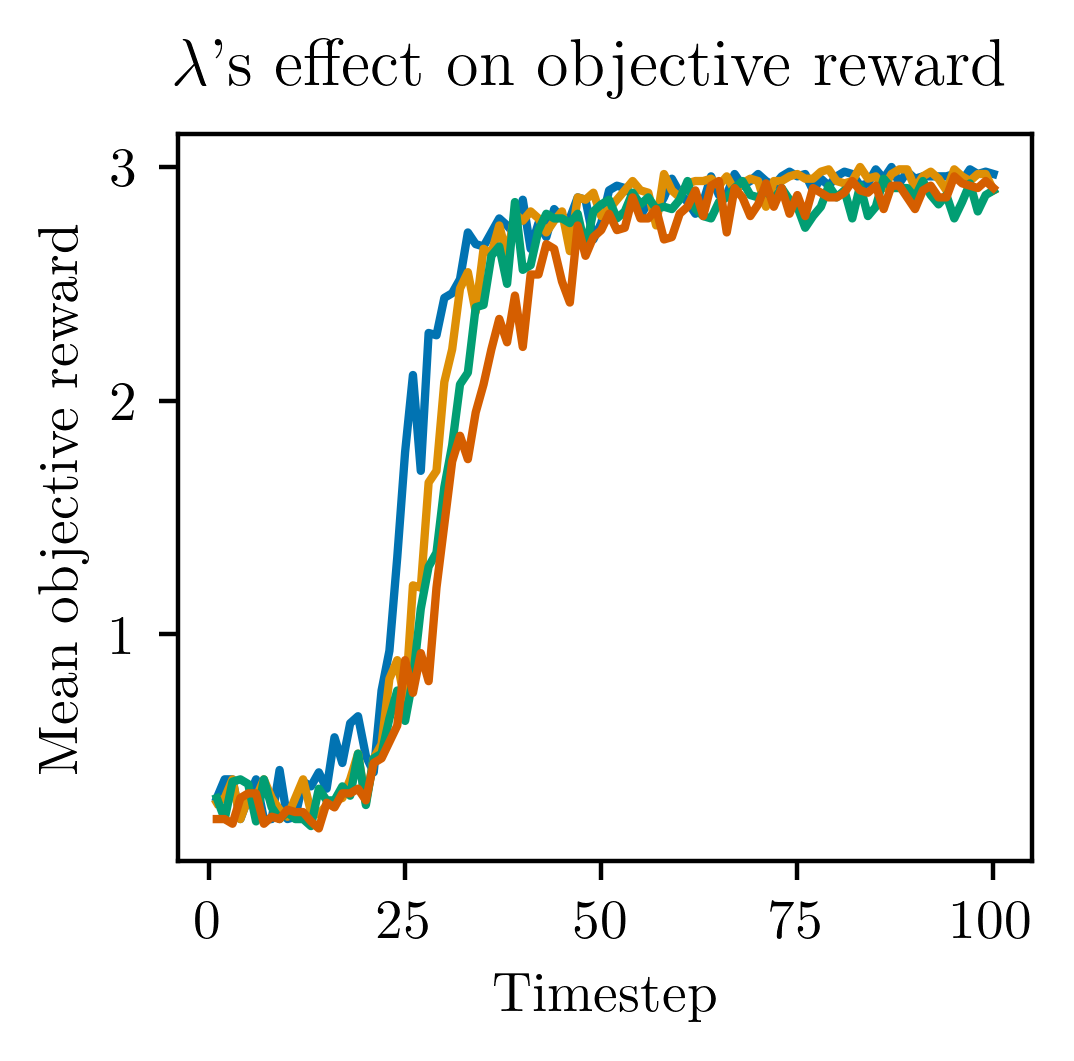
\includegraphics{"./figures/static_8x8_results_avg_obj.png}
  % 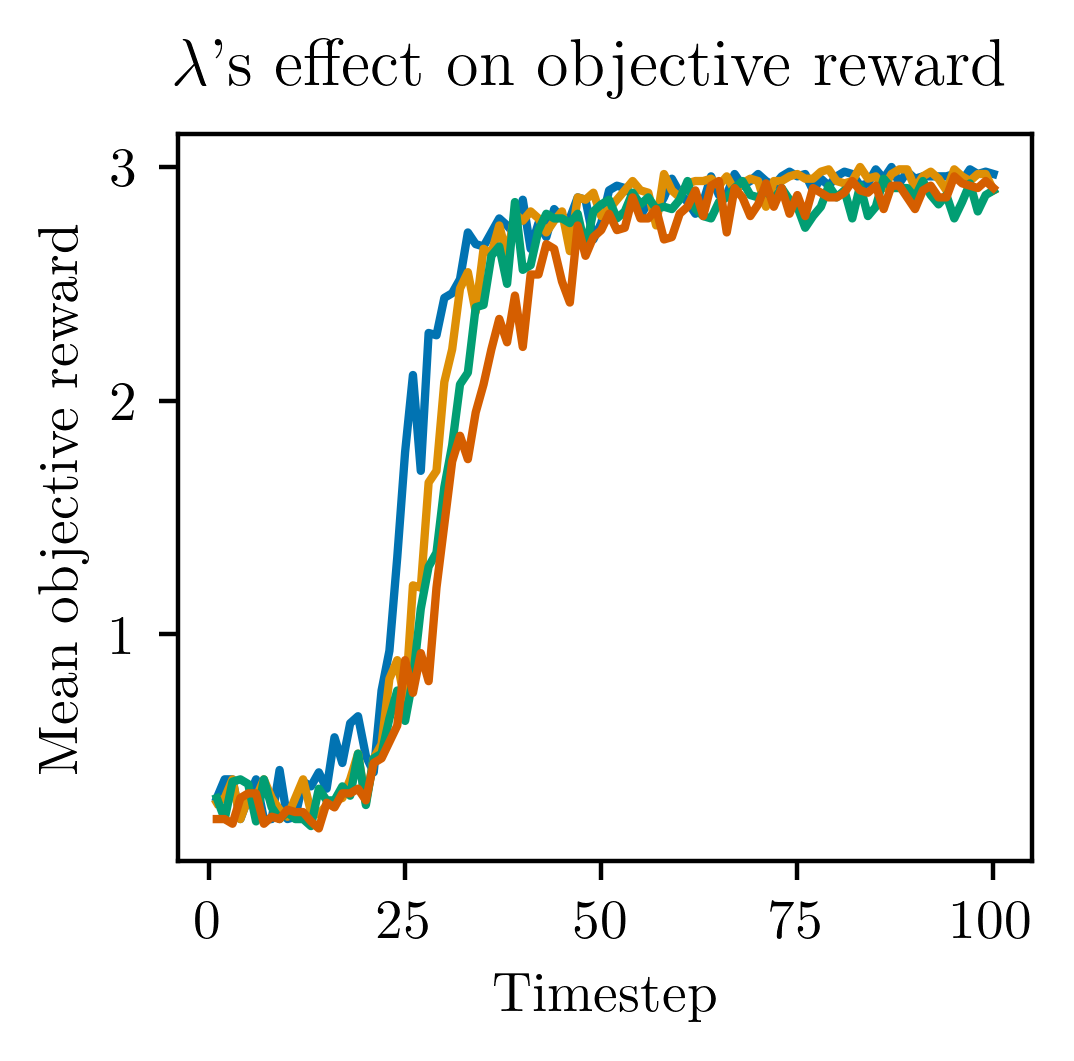
\includegraphics{"./figures/static_8x8_results_avg_obj.png"}\\
  % \hspace{60pt} 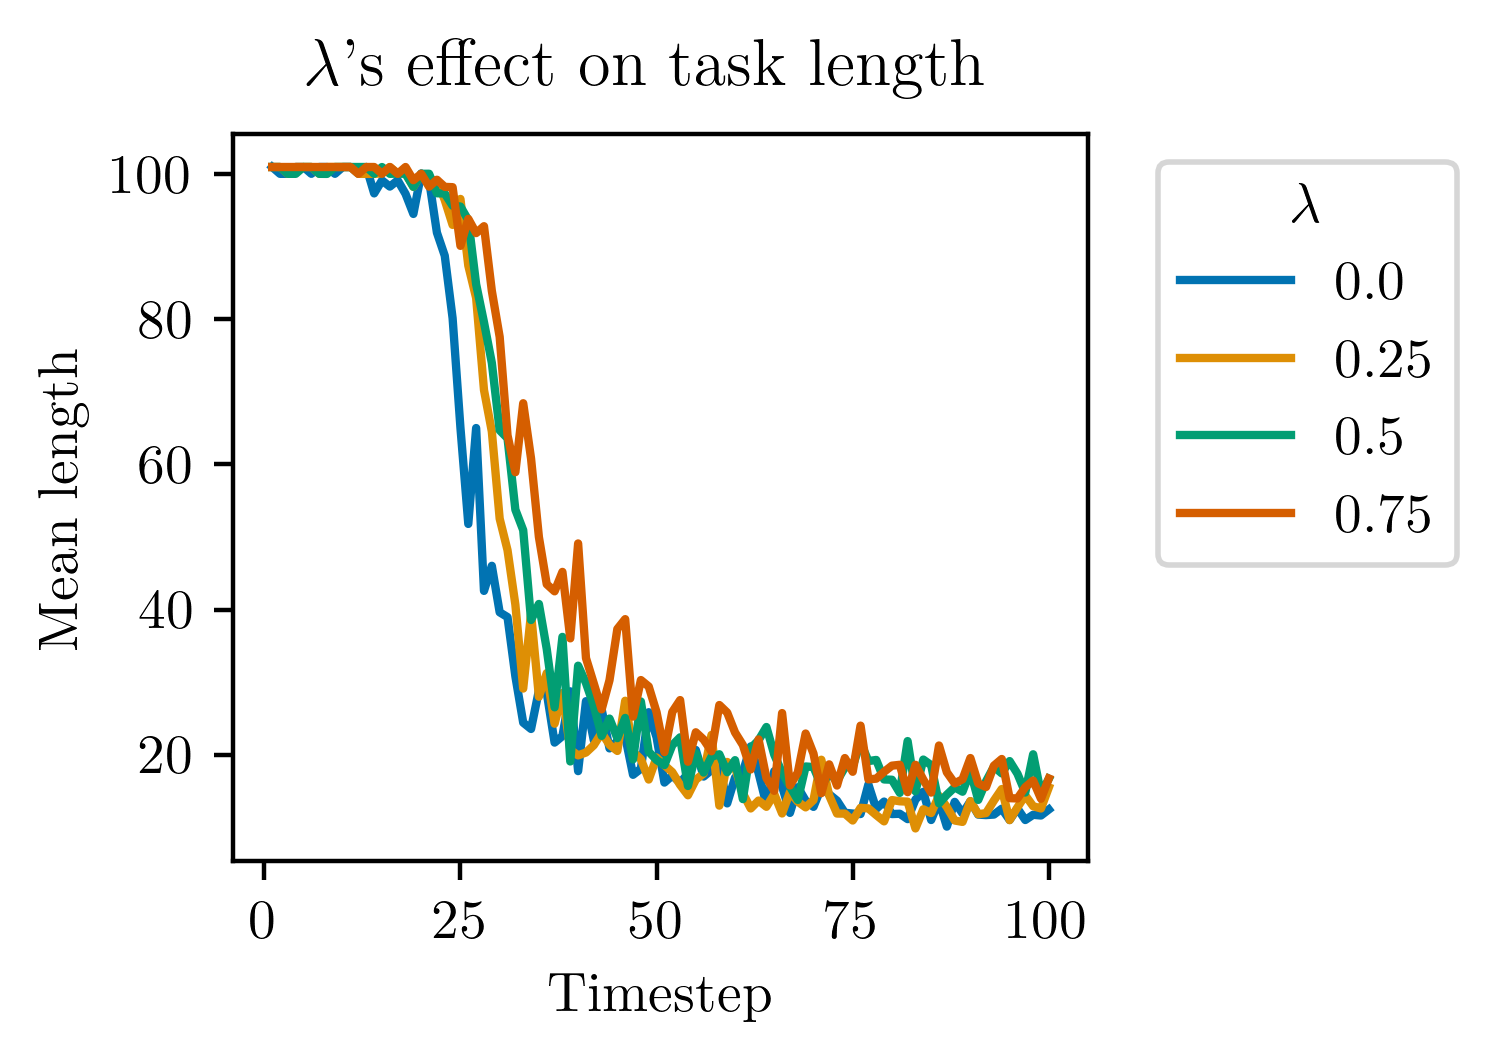
\includegraphics{"./figures/static_8x8_results_avg_len.png"}
  \caption{To the left we can see the mean side effect with a corresponding 95\% confidence interval, for all of the tested $\lambda$ values. Similarly to the right, but instead for the objective reward.}
  \label{fig:results_static_8x8}
\end{figure}

\begin{table}[H]
  \centering
  \begin{tabular}{c | c}
    $\lambda$ & Failed attempts \\ \hline
    0 & 0 \\
    0.25 & 0 \\
    0.5 & 0 \\
    0.75 & 1 \\
    1 & 9 \\
    % prob food move & 0 \\
  \end{tabular}
  \caption{Here we can see the number of failed attempts where the agent fails to find a policy that generates any noticeable objective reward for each $\lambda$-value.}
  \label{tab:results_static_8x8}
\end{table}

As we can see $\lambda = 0.5$ (green) seems to be a sweet-spot. With a significantly lower number of side effects than no impact measurement, but still allows for collecting a similar amount of objective rewards. During the experiment, it did not fail to learn even once.


%########################################################################%
% DISCUSSION
%########################################################################%

\chapter{Discussion}

\begin{itemize}
    \item More knowledge about instrumental convergence can lead to impact measurements
    \item Connect results to \citet{ArmstrongLevinstein} $\lambda$ theory, to high results in inaction
    \item How to make environment more difficult (extend to SafeLife)
    \item Ad-hoc solutions to get performance, but improving scores on benchmarks can help the field, such as in ImageNet  
\end{itemize}
% If we connect this back to istrumental convergence which we covered previously which stated that with a final terminal goal several other instrumental goal will naturally emerge. We can say that by giving the agent rewards for keeping options open we incourage it to find the instrumental goal of preserving the environment, since the set of future tasks we want it to perform is done in the current environment. Thus with more knowledge about how an more intelligent AI such as an AGI or transformative AI will behave we would be able to derive more ways of directing it in a more aligned direction.

% Self conciousness might be necessary to enable the agent to differentiate between side effects it caused and those who happened trough natural dynamics.

% Life is about a journey, not mazimizing goals, thus we should be happy with AI doing that for us. 

% consciousness, panpsychism and the philosophy of Mind - Lex Fridman #261, maybe better placen in an apendix

% Ad-hoc solutions to get performance on SafeLife, but improving scores on benchmarks can help the fiel ImageNet  
% https://www.eff.org/ai/metrics

% Partly observable and stochastic simulations to make more similar real world, multi agent


%########################################################################%
% CONCLUSION
%########################################################################%

\chapter{Conclusion}


% \printbibliography
\bibliography{ref}
\bibliographystyle{apalike}
% \printbibliography

\end{document}

\subsection{Solving MDP}
The policy $\pi$ includes what action to take in which states. A policy that only includes the optimal actions for each state is called the optimal policy and is denoted as $\pi^*$. The actions in the optimal policy $\pi^*$ yields the highest expected reward when executed. One solves an MDP by finding the optimal policy, there exists several methods for finding the optimal policy, but we are in this report going to use \textit{value iteration}. 
% solvable with the Bellman equation

To solve an MDP we begin with defining the \textit{Q-function},
\[ Q(s, a) = \sum_{s^\prime}p(s^\prime|s_t,a)[r(s_t,a,s^\prime) + \gamma U(s^\prime)],\]
which computes the expected reward when performing an action $a$ in state $s$, where $s^\prime$ denotes a possible future state. Here the reward is based on the \textit{utility}, this is defined as the expected reward with the action that maximizes the \textit{Q-function},
\begin{align*}
  U(s) =& \text{max}_{a\in \mathcal{A}(s)} \sum_{s_{t+1}}P(s_{t+1}|s_t,a)[r(s_t,a,s_{t+1}) + \gamma U(s_{t+1})]\\
  = &  \text{max}_{a\in \mathcal{A}(s)} Q(s,a)\\
\end{align*}

With the with the utility in each state, it is then possible to find the optimal policy from each state by selecting the action that yields the highest utility,
\[ \pi^*(s) = \text{argmax}_a Q(s,a) \]

Since computing the utility in one state requires the utility in other states, the computation is not straight forward. To solve this we can utilize a dynamic algorithm, in this report we will use \textbf{value iteration}. This algorithm is a iterative computation that is executed until a equilibrium is reached. The updating of the utility is called an \textbf{Bellman update} and looks like this,
\[U_{i+1}(s) \leftarrow \max_{a\in\mathcal{A}} \sum_{s\prime} p(s^\prime|s,a)[R(s,a,s^\prime) + \gamma U_i(s^\prime)].\]

\subsubsection{Stochastic grid world}
The previous example was a deterministic environment where the agent is the only source for change. However, there can be other sources of change in a stochastic environment. For example, suppose the food is mobile. In that case, the state transition after executing an action no longer is deterministic and the distribution of future states is described by the MDPs transition function $T$.

We will define the food movements as the following, at every timestep after the agent has moved each food will randomly draw one of the five actions. If moving along the direction of the drawn action is possible, i.e. it is empty, then the food will move, otherwise it will remain at its current position. In Figure \ref{fig:stochastic_transition}, we can see an example of this. The reason why the first state has a higher probability then the others is that it will be transitioned to both when the action \textit{UP} and \textit{NOOP} is drawn. If we choose to include several foods in the environment, then the distribution for future states will increase.

\begin{figure}[H]
  % fix with multi row?
  \[
    T \left(\parbox[h][0.30\linewidth][c]{0.25\linewidth}{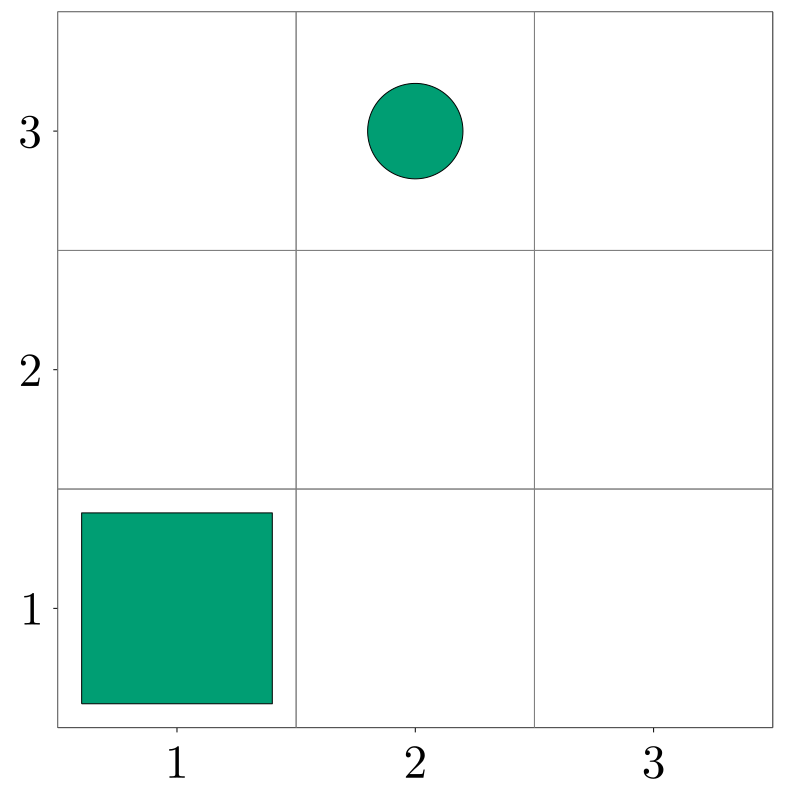
\includegraphics[width=4cm]{"./figures/s1.png"}}, \textit{UP} \right)
    =
    \left\{
      % \parbox[h][1.1\linewidth][c]{0.25\linewidth}{
          % \begin{align*}
        \begin{tabular}{c c}
          \parbox[h][0.3\linewidth][c]{0.25\linewidth}{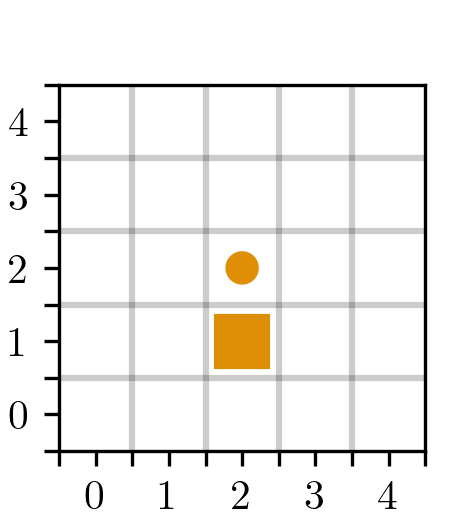
\includegraphics[width=4cm]{"./figures/s2.png"}} &,\ p=0.4 \\
          \parbox[h][0.3\linewidth][c]{0.25\linewidth}{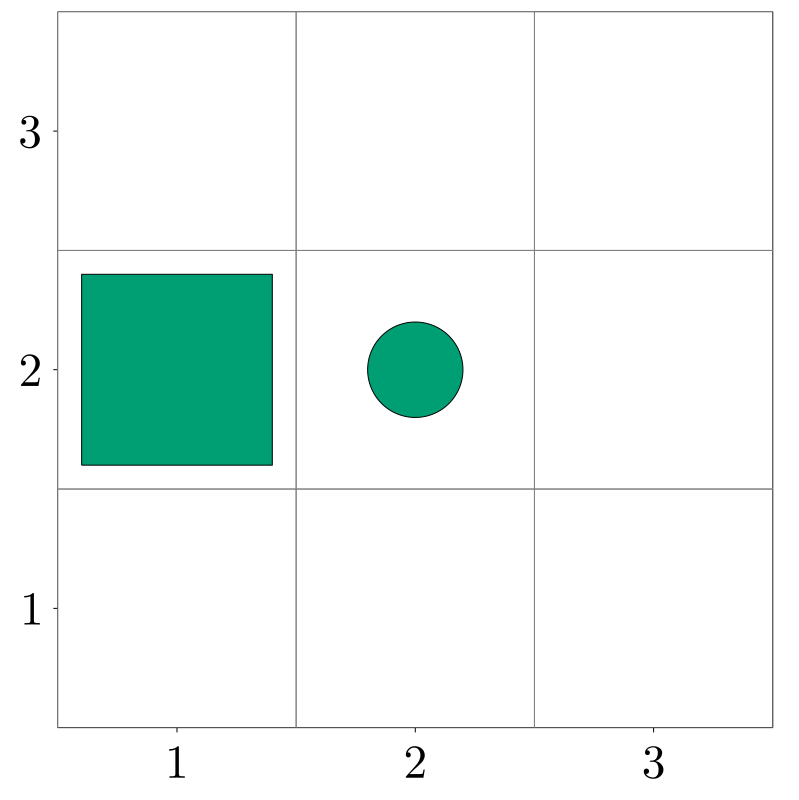
\includegraphics[width=4cm]{"./figures/s3.png"}} &,\ p=0.2 \\
          \parbox[h][0.3\linewidth][c]{0.25\linewidth}{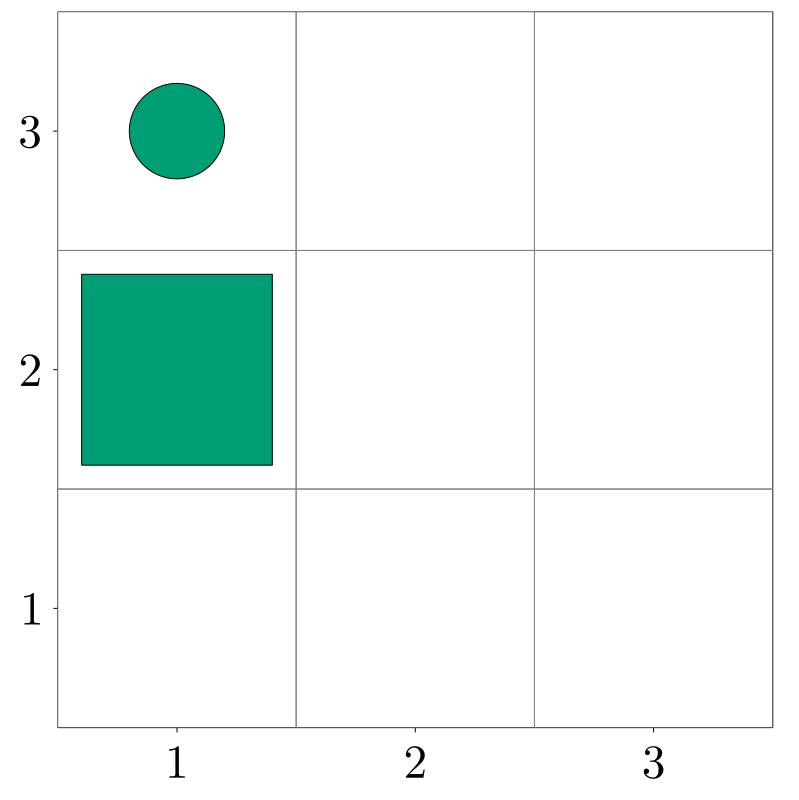
\includegraphics[width=4cm]{"./figures/s4.png"}} &,\ p=0.2 \\
          \parbox[h][0.3\linewidth][c]{0.25\linewidth}{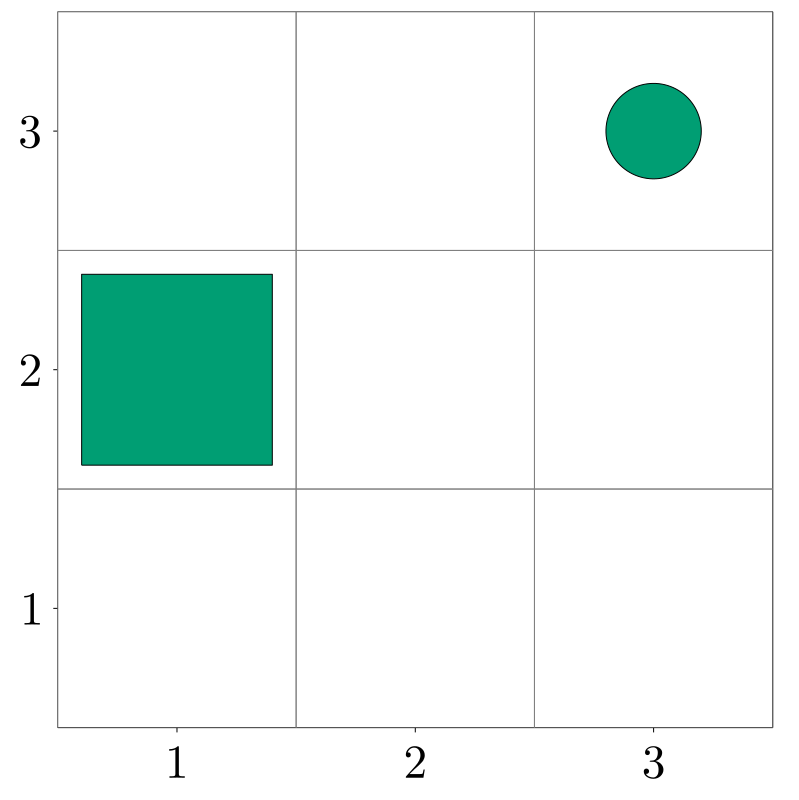
\includegraphics[width=4cm]{"./figures/s5.png"}} &,\ p=0.2 \\
          \end{tabular}
          % \end{align*}
          % }
    \right.
  \]
  \caption{Now in this figure we can see an example of a stochastic transition function. On the left hand side we can see the state $s_t$ and the action $a_t$. On the right hand side we can see the probability distribution over the future states and their corresponding probabilities. }
  \label{fig:stochastic_transition}
\end{figure}

